\documentclass[titlepage]{jsarticle}
\usepackage[utf8]{inputenc}
\usepackage{amsmath}
\usepackage{bm}
\usepackage{otf}
\usepackage{comment}
\usepackage[dvipdfmx]{graphicx}
\usepackage{multirow}
\usepackage{mathcomp}
\usepackage{textcomp}
\usepackage{longtable}
\usepackage{comment}
\usepackage[dvipdfmx]{hyperref}
\usepackage{enumerate}

\usepackage{subcaption}

\title{物理学実験\ajRoman{2}レポート(顕微鏡光学系1A)}
\author{理学部物理学科 05-211525 齋藤駿一\\
共同実験者:河野匡 ソンテスン}
\date{\today 提出}

\begin{document}

\maketitle

\section{実験0}
まず光軸の高さと向きを調整した.

\subsection{手法}
\begin{figure}[htbp]
    \centering
    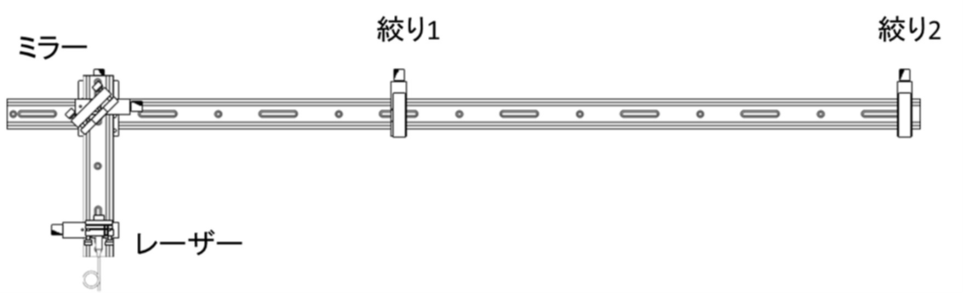
\includegraphics[width=10cm]{exp0.png}
    \caption{光学素子の配置(実験0)}
    \label{fig:exp0}
\end{figure}

まず図\ref{fig:exp0}のようにレール上に光学素子を配置した.
絞り1,2の高さはともに約120\,mmに調整し,その間の距離は十分長くとった.
このとき光軸がレール上の高さ約120\,mmで水平を保つためには,絞り1,2を閉じたときでもレーザーが絞り2の中央を通り抜ければ良い.
そこで次の手順に従って光軸を調整した.
\begin{enumerate}
    \item 絞り1,2をともに閉じた.
    \item レーザーヘッドの向きを調整し,レーザーが絞り1の中央を通過するようにした.
    \item 絞り1を開いた.
    \item ミラーの向きを調整し,レーザーが絞り2の中央を通過するようにした.
    \item 絞り1を閉じ,上の操作を10回ほど繰り返した.
\end{enumerate}

\subsection{結果}
レーザーがミラーに反射して絞り1,2の両方の中央を通過することが確認できた.

\section{実験1}
レンズの公式を実験により検証した.

\subsection{原理}
\subsubsection{ABCD行列}
レンズの公式を導くにあたってABCD行列法を用いる.
まず媒質の屈折率を$n$,ある地点での光線の光軸からの高さを$x$,傾きを$u$とするとき,$p=nu$を用いてその地点での光線を光線ベクトル$^t(x,p)$で表す.
次に光学系を通過することによる光線ベクトルの遷移を考える.
たとえば光線$^t(x,p)$が屈折率$n$の媒質中を距離$z$だけ直進して$^t(x',p')$に変化したとする.
このとき光線は直進するので二つのベクトルの間には次の関係がある:
\begin{equation}
    \left(
    \begin{array}{c}
        x' \\
        p'
    \end{array}
    \right)=\left(
    \begin{array}{cc}
        1 & z/n \\
        0 & 1
    \end{array}
    \right)\left(
    \begin{array}{c}
        x  \\
        p 
    \end{array}
    \right) \label{straight}
\end{equation}
別の場合として,屈折率1の媒質中で光線$^t(x,p)$が焦点距離$f$の薄い凸レンズを通過して$^t(x,p)$に変化したときを考える.
光線が光軸に十分近い場合,$^t(x',p')$は$^t(x,p)$に対して線形に変化すると考えられる(近軸近似)ので,これらの関係は先ほどのように行列で書ける.
その上でレンズの性質として具体的に
\begin{itemize}
    \item 平行光は後側焦点を通過する向きに屈折する
    \item レンズの中心を通る光は直進する
\end{itemize}
の二点を考えると,次の式が導かれる:
\begin{equation}
    \left(
    \begin{array}{c}
        x' \\
        p'
    \end{array}
    \right)=\left(
    \begin{array}{cc}
        1 & 0 \\
        -1/f & 1
    \end{array}
    \right)\left(
    \begin{array}{c}
        x  \\
        p 
    \end{array}
    \right) \label{lens}
\end{equation}
このように近軸近似の下では一般に光学系は光線ベクトルに作用する行列として表せる.
この行列を光学系のABCD行列と呼ぶ.

\subsubsection{結像関係式とレンズの公式}
光学系の入射面から距離$a$だけ前方に高さ$x$の物体があり,光学系の最終面から距離$b$だけ後方にスクリーンがあるとする.
ただし媒質の屈折率は1とし,光学系のABCD行列は
\begin{equation}
    \left(
    \begin{array}{cc}
        A & B \\
        C & D
    \end{array}
    \right)
\end{equation}
とする.
物体の先端から発された光線$^t(x,p)$が最終的にスクリーンで$^t(x',p')$となると考えると,これは式\eqref{straight}を用いて
\begin{align}
    \left(
    \begin{array}{c}
        x' \\
        p'
    \end{array}
    \right)&=\left(
    \begin{array}{cc}
        1 & b \\
        0 & 1
    \end{array}
    \right)\left(
    \begin{array}{cc}
        A & B \\
        C & D
    \end{array}
    \right)\left(
    \begin{array}{cc}
        1 & a \\
        0 & 1
    \end{array}
    \right)\left(
    \begin{array}{c}
        x  \\
        p 
    \end{array}
    \right) \notag\\
    &=\left(
    \begin{array}{cc}
        A + Cb & Aa + B + Cab + Db \\
        C & Ca + D
    \end{array}
    \right)\left(
    \begin{array}{c}
        x  \\
        p 
    \end{array}
    \right)
\end{align}
と書ける.
物体から出た光線がスクリーン上で結像する条件は$x'$が$p$によらないこと,すなわち
\begin{equation}
    b = -\frac{Aa+B}{Ca+D}
\end{equation}
が成り立つことである.
この式を結像関係式と呼ぶ.
たとえば光学系として焦点距離$f$の薄いレンズをとると,式\eqref{lens}から結像関係式は
\begin{align}
    &b = - \frac{a}{-a/f + 1} \notag\\
    &\frac{1}{a} + \frac{1}{b} = \frac{1}{f} \label{abf}
\end{align}
となる.
これはレンズの公式と呼ばれる.

\subsubsection{複合レンズの主点}
焦点距離$f_1$のレンズと焦点距離$f_2$のレンズが距離$d$を隔てて置かれた光学系を考える.
媒質の屈折率を1とすると,この光学系のABCD行列は
\begin{equation}
    \left(
    \begin{array}{cc}
        1 & 0 \\
        -1/f_1 & 1
    \end{array}
    \right)\left(
    \begin{array}{cc}
        1 & d \\
        0 & 1
    \end{array}
    \right)\left(
    \begin{array}{cc}
        1 & 0 \\
        -1/f_2 & 1
    \end{array}
    \right)=\left(
    \begin{array}{cc}
        1-d/f_1 & d \\
        -1/f_1 - 1/f_2 +d/(f_1f_2) & 1 - d/f_2 
    \end{array}
    \right) \label{2lens_1}
\end{equation}
となる.
一方で光が距離$\delta_1$だけ直進してから焦点距離$f$のレンズにより屈折し,その後距離$\delta_2$だけ直進する光学系を考える.
媒質の屈折率を1とすると,この光学系のABCD行列は
\begin{equation}
    \left(
    \begin{array}{cc}
        1 & \delta_2 \\
        0 & 1
    \end{array}
    \right)\left(
    \begin{array}{cc}
        1 & 0 \\
        -1/f & 1
    \end{array}
    \right)\left(
    \begin{array}{cc}
        1 & \delta_1 \\
        0 & 1
    \end{array}
    \right)=\left(
    \begin{array}{cc}
        1-\delta_2/f & \delta_1 + \delta_2 - \delta_1\delta_2/f \\
        -1/f & 1 - \delta_1/f 
    \end{array} \label{2lens_2}
    \right)
\end{equation}
となる.
これら二つの行列\eqref{2lens_1},\eqref{2lens_2}は次のようにパラメータを定めれば完全に一致する:
\begin{align}
    \frac{1}{f} &= \frac{1}{f_1} + \frac{1}{f_2} - \frac{d}{f_1f_2} \label{df}\\
    \delta_1 &= \frac{f}{f_2}d \label{dd1}\\
    \delta_2 &= \frac{f}{f_1}d \label{dd2}
\end{align}
つまり二枚のレンズからなる光学系はそれと等価な単一レンズの光学系に置き換えることができる.
この置き換えをレンズの合成と呼び,置き換わった先の単一レンズを合成レンズと呼ぶ.

しかし単純なこの置き換えだけでは光学系の長さが$d$から$\delta_1+\delta_2$へと変化してしまう.
そこで二枚のレンズの光学系において,レンズ1から後方に$\delta_1$進んだ位置とレンズ2から前方に$\delta_2$戻った位置それぞれにおいて光軸に垂直な平面を仮定する.
そして前側の平面に達した光線$^t(x,p)$は後側の平面で光線$^t(x',p')$となって放出されると考える.
ただし$^t(x',p')$は単一レンズによる変換を表す式\eqref{lens}によって決まるとする.
この平面は合成レンズの入射面と最終面を表しており,平面と光軸の交点を主点と呼ぶ.
本レポートでは前側の平面と光軸の交点を前側主点,後側の平面と光軸の交点を後側主点と呼ぶことにする.

二枚のレンズからなる光学系の結像関係式は,レンズの合成によって簡単に得られる.
たとえば前側主点から距離$s$だけ前方に物体があり,後側主点から距離$s'$だけ後方にスクリーンがあるとすると,結像関係式は合成レンズに関するレンズの公式\eqref{abf}から
\begin{equation}
    \frac{1}{s_1} + \frac{1}{s_2} = \frac{1}{f} \label{ssf}
\end{equation}
で与えられる.

\subsection{手法}
\subsubsection{単レンズ}
\begin{figure}
    \centering
    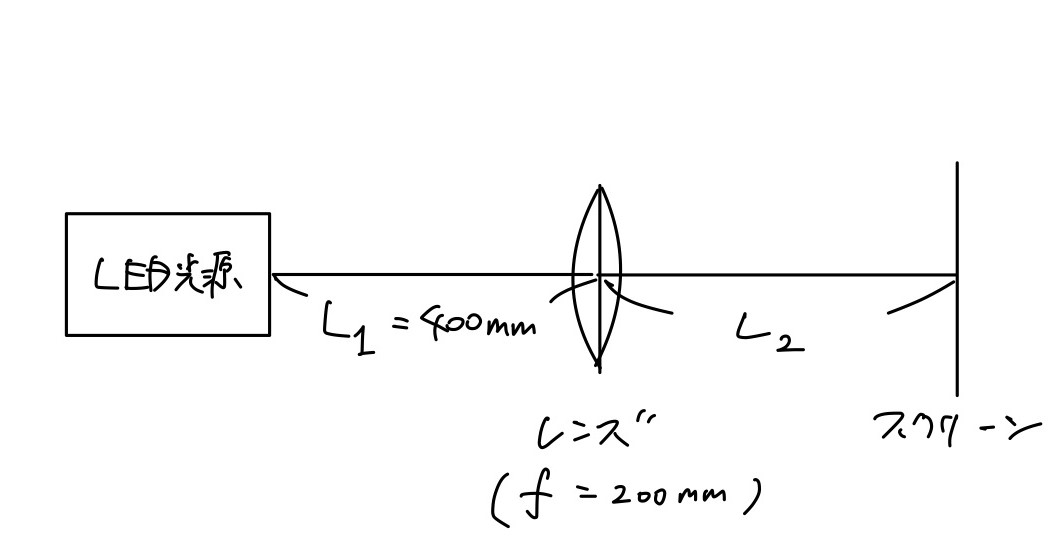
\includegraphics[width=10cm]{single.jpg}
    \caption{単レンズの光学系}
    \label{fig:single}
\end{figure}

実験0の後レーザーの電源を切ってミラーと絞り1,2を除き,図\ref{fig:single}のようにレンズ(焦点距離200\,mm)とスクリーンをレール上に配置した.
まず$L_1$の値を400\,mmに調整し,LED光源の模様がスクリーンに結像するようにスクリーンの位置を調整した.
このときの光源からスクリーンまでの距離$L$を記録し,次式によりレンズからスクリーンまでの距離$L_2$を求めた.
\begin{equation}
    L_2 = L - L_1
\end{equation}
次に$L_1$の値を300\,mm,600\,mmに調整し,それぞれの場合における$L_2$の値を記録した.
最後にこれらの結果とレンズの公式から導かれる結果を比較した.

\subsubsection{複合レンズ}

\begin{figure}
    \centering
    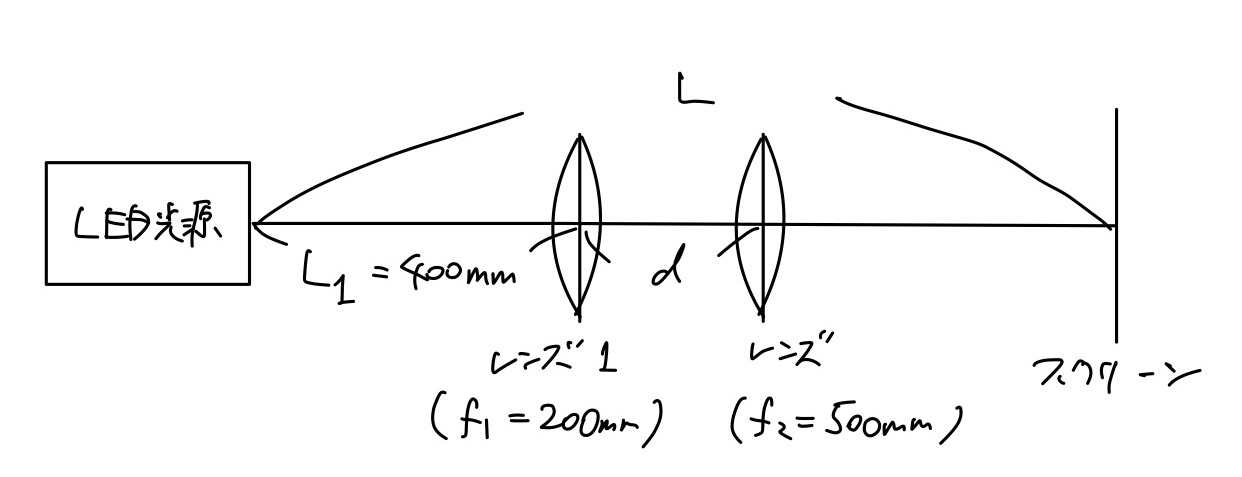
\includegraphics[width=10cm]{double.jpg}
    \caption{複合レンズの光学系}
    \label{fig:double}
\end{figure}

先ほどの実験に引き続き,図\ref{fig:double}のようにレンズ2枚(レンズ1,レンズ2の焦点距離$f_2$はそれぞれ200\,mm,500\,mm)とスクリーンをレール上に配置した.
ここで光源からレンズ1までの距離$L_1$の値を400\,mmに固定した.
まずレンズ1とレンズ2の間の距離$d$の値を100\,mmに調整し,光源の模様がスクリーンに結像するようにスクリーンの位置を調整した.
このとき光源からスクリーンまでの距離$L$を記録した.
次に$d$の値を20\,mm(レンズ1,2のレンズホルダーが密着した状態),200\,mmに調整してそれぞれの$L$を記録した.

\subsection{結果}
単レンズと複合レンズの場合の測定結果はそれぞれ表\ref{tab:single_lens},表\ref{tab:double_lens}のようになった.

\begin{table}[htbp]
    \centering
    \caption{光源からレンズまでの距離$L_1$とレンズから結像位置までの距離$L_2$の関係(単レンズ)}
    \label{tab:single_lens}
    \begin{tabular}{c|cc|c}
        $L_1$(mm) & $L$(mm) & 測定値$L_2$(mm) & 理論値$L_2$(mm) \\
        \hline\hline
        400 & 800 & 400 & 400\\
        300 & 905 & 605 & 600\\
        600 & 895 & 295 & 300\\
        \hline
    \end{tabular}
\end{table}

\begin{table}[htbp]
    \centering
    \caption{光源からレンズまでの距離$L_1$と光源から結像位置までの距離$L$の関係(複合レンズ)}
    \label{tab:double_lens}
    \begin{tabular}{c|cccc|c}
        $d$(mm) & $f$(mm) & $\delta_1$(mm) & $\delta_2$(mm) & 測定値$L$(mm) & 理論値$L$(mm) \\
        \hline\hline
        100 & 167 & 33.3 & 83.3 & 685 & 688\\
        20 & 147 & 5.9 & 14.7 & 640 & 636\\
        200 & 200 & 80 & 200 & 745 & 743\\
        \hline
    \end{tabular}
\end{table}

\subsection{考察}
\subsubsection{単レンズ}
単レンズによって光源の模様がスクリーンで結像している場合を考える.
このとき光源からレンズまでの距離$L_1$とレンズからスクリーンまでの距離$L_2$はレンズの公式\eqref{abf}から
\begin{equation}
    \frac{1}{L_1} + \frac{1}{L_2} = \frac{1}{f}
\end{equation}
を満たす.
この式から導かれる結果と実験結果を比較すると,表\ref{tab:single_lens}のようになる.
レンズやスクリーンの位置の測定には約5\,mmの測定誤差があったので,$L_2$の測定値と理論値は一致したといえる.

\subsubsection{複合レンズ}
複合レンズの場合,それらの合成レンズを用いて結像位置を考えることができる.
具体的にはまず式\eqref{df}を用いて合成レンズの焦点距離を導き,式\eqref{dd1},式\eqref{dd2}を用いて合成レンズの主点の位置を導く.
次に光源と前側主点の間の距離を$s$,後側主点とスクリーンの間の距離を$s'$とすると
\begin{equation}
    s = L_1 + \delta_1
\end{equation}
が成り立ち、これと結像関係式\eqref{ssf}から$s'$が計算できる.
以上で導いたパラメータを用いると,光源からスクリーンまでの距離$L$は
\begin{equation}
    L = s_1 + s_2 + (d - \delta_1 - \delta_2)
\end{equation}
で与えられる.
この式から導かれる$L$の理論値と実験で得られた$L$の測定値を比較すると,表\ref{tab:double_lens}のようになる.
これらの差は測定誤差5\,mm以内に収まっているので,実験結果は理論と整合していたといえる.

\subsubsection{複雑な複合レンズ}
今回実験で扱った複合レンズは単純だったが,実際にはさらに複雑にレンズが組み合わさった光学系を扱うことがある.
その場合には先ほどの考察のように主点位置を求めることが難しいため,主点位置を求めずに結像位置を求める方法が望ましい.
ここではまずその際に有用なニュートンの式を導く.

まずパラメータ$t$,$t'$を
\begin{align}
    s &= f + t \\
    s' &= f + t'
\end{align}
となるように定義する.
具体的には$t$は物体から前側焦点までの距離を,$t'$は後側焦点からスクリーンまでの距離を表す.
このとき結像関係式\eqref{ssf}は
\begin{equation}
    \frac{1}{f+t} + \frac{1}{f+t'} = \frac{1}{f}
\end{equation}
となり,これを整理すると次式が得られる:
\begin{equation}
    tt' = f^2
\end{equation}
これをニュートンの式と呼ぶ.

ニュートンの式を用いると結像位置は次のように理解できる.
まず前側(後側)焦点の位置は,光学系の後方(前方)から平行光を入射させるとその集光点として実験的に分かる.
そこで光源から前側焦点までの距離$t$を測れば,ニュートンの式から後ろ側焦点からスクリーンまでの距離$t'$が分かる.
こうして主点の位置を求めずに結像位置が求まる.

\section{実験2}
ここではレーザー光をレンズで集光したときのスポットサイズを計測し,回折による影響を考察する.

\subsection{原理}
\subsubsection{レンズによる集光}
平行光が焦点距離$f$のレンズを通過する場合の回折効果について述べる.
レンズの置かれた平面を$x-y$座標で表し,スクリーンの置かれた平面を$x'-y'$座標で表す.
ここではこの平面間の距離はレンズの焦点距離$f$に等しい(スクリーン上で集光する)とする,
またレンズのある領域$D$を関数
\begin{equation}
    g(x,y) = \left\{\begin{array}{ll}
        1 & (x,y)\in D \\
        0 & (x,y)\notin D
    \end{array}\right.
\end{equation}
で表す.
ただしレンズの場合,平行光が入射したとき後側焦点で位相が揃うことから,
\begin{equation}
    r' = \sqrt{f^2 + x^2 + y^2}
\end{equation}
を用いると,点$(x,y)$に来た入射波には位相因子
\begin{equation}
    h(x,y) = \exp{(-ik(r'-f))}
\end{equation}
がかかって位相が$k(r'-f)$だけ進むことが分かる.

ホイヘンスの原理により,この$D$上の各点に光源が存在しておりスクリーンにはこれらの作る光の重ね合わせが現れると考えることができる.
よってスクリーン上での強度分布は次の式で与えられる:
\begin{align}
    u(x',y') &= \frac{1}{i\lambda} \iint g(x,y)h(x,y) \frac{A\exp{(ikr)}}{r} dxdy \notag\\
    &= \frac{1}{i\lambda} \iint g(x,y) \frac{A\exp{(ik(r-r'+f))}}{r} dxdy
\end{align}
ここで
\begin{equation}
    r = \sqrt{f^2 + (x-x')^2 + (y-y')^2}
\end{equation}
とした.
とくに$x^2 + y^2 \ll f$かつ$(x-x')^2 + (y-y')^2 \ll f$のとき,$r$および$r'$は次のように原点まわりでテイラー展開できる:
\begin{align}
    r &\approx f + \frac{(x-x')^2 + (y-y')^2}{2f} \\
    r' &\approx f + \frac{x^2 + y^2}{2f} 
\end{align}
このとき強度分布は
\begin{align}
    u(x',y') &= \frac{A}{if\lambda}\exp{\left(ik\frac{x'^2 + y'^2}{2f}\right)} \iint g(x,y) \exp{\left(-i\frac{k(x'x + y'y)}{f}\right)}dxdy \notag\\
    &= A'\iint g(x,y) \exp{\left(-i\frac{k(x'x + y'y)}{f}\right)} dxdy \label{foulier}
\end{align}
のように,$g(x,y)$のフーリエ変換を用いて書ける.
ただし
\begin{equation}
    A' = \frac{A}{if\lambda}\exp{\left(ik\frac{x'^2 + y'^2}{2f}\right)} 
\end{equation}
とした.

\subsubsection{円形レンズの回折限界}
式\eqref{foulier}を用いると円形のレンズによる集光点でのスポット径が分かる.
円形レンズを通過するレーザーの半径を$R$とし,$(x,y)$と$(x',y')$をそれぞれ極座標$(\rho,\theta)$,$(\rho',\theta')$に変換すると,
\begin{align}
    u(\rho',\theta') &= A'\int_0^R \rho d\rho \int_0^{2\pi} d\theta \exp{\left(-i\frac{k\rho'\rho}{f}(\cos{\theta'}\cos{\theta}+\sin{\theta'}\sin{\theta})\right)} \notag\\
    &= A' \int_0^R \rho d\rho \int_0^{2\pi} d\theta \exp{\left(-i\frac{k\rho'\rho}{f}\cos{(\theta'-\theta)}\right)} \notag\\
    &= A' \int_0^R d\rho \,2\pi\rho J_0\left(\frac{k\rho'\rho}{f}\right) \notag\\
    &= 2\pi A' \int_0^{kR\rho'/f} \frac{f}{k\rho'}dz \, \frac{f}{k\rho'}z J_0(z) \qquad \left(z = \frac{k\rho'}{f}\rho \right)\notag\\
    &= 2\pi A' \left(\frac{f}{k\rho'}\right)^2 \frac{kR\rho'}{f} J_1\left(\frac{kR\rho'}{f}\right) \notag\\
    &= 2\pi R^2 A' \frac{J_1\left(\frac{kR\rho'}{f}\right)}{\frac{kR\rho'}{f}} \notag\\
    &\propto \frac{2J_1\left(\frac{kR\rho'}{f}\right)}{\frac{kR\rho'}{f}} \label{bessel}
\end{align}
この変形の際,ベッセル関数の性質
\begin{align}
    &J_0(z) = \frac{1}{2\pi} \int_0^{2\pi} d\theta \exp{(-iz\sin{\theta})} = \frac{1}{2\pi} \int_0^{2\pi} d\theta \exp{(-iz\cos{\theta})} \\
    &\frac{d}{dz}(z^n J_n(z)) = x^n J_{n-1} (z)
\end{align}
を用いた.
ここでベッセル関数$J_1(x)$の最初のゼロ点は$x\approx3.83$にあることから,スクリーン上のスポット径$r$は
\begin{equation}
    \frac{kRr}{f} = \frac{2\pi Rr}{f\lambda} = 3.83
\end{equation}
より
\begin{equation}
    r = \frac{3.83}{2\pi} \frac{f\lambda}{R} \approx 0.61\frac{f\lambda}{R} \label{limit}
\end{equation}
と計算できる.
こうして理論的に集光点でのスポット径が得られた.

\subsection{手法}
\subsubsection{アフォーカル光学系の設置}
まずレーザー光(スポット径2.9\,mm)を拡大するためのアフォーカル光学系を組んだ.
ここではレンズ1(焦点距離$-50$\,mm)とレンズ2(焦点距離$750$\,mm)を距離700\,mmだけ離して配置した.
このときレンズの凸面(凹面)が平行光側を向くよう注意した.
またレンズ2の後側でスクリーンを前後させて平行光になっている(スポットの位置と大きさが概ね一定である)ことを確認し,スクリーン上でのスポット径を定規で計測した.

\subsubsection{レンズとカメラの設置}
次にレンズによる集光点をカメラで撮影する光学系を次の手順で組んだ.
まずアフォーカル光学系の後側に絞り(半径$R$)を置き,そのさらに後側にレンズ3(焦点距離500\,mm)を置いた.
次にレンズ3の後側にスクリーンを置いて集光点を確認してから,スクリーンのかわりにカバー付きのカメラを置き,カバーの中央に集光点が来るようにした.
そしてレーザーヘッドの前に減光フィルター(10\%,1\%,0.1\%の3種類)をセットし,スポットが肉眼で見えないくらいに減光してから,カメラのカバーを外してスポットの画像を確認した.
その後カメラを前後させて,この画像上でピクセルの輝度値が最も高くなる位置(光が最も集中する位置)に調整した.
またカメラの向きを調整してスポットが画像の中央付近に来るようにした.

\subsubsection{スポット径の計測}
最後にカメラでスポットを撮影した画像をもとに,次の手順でスポット径を計測した.
まず絞りの直径を$2R=20$\,mmとし,次のいずれかの調整を行ってピクセルの輝度値が200以上になるようにした.
\begin{itemize}
    \item レーザーヘッド前の減光フィルターのいずれかを外す.
    \item すでに外したレーザーヘッド前の減光フィルターのいずれかを戻す.
    \item カメラの露光時間を変える.
\end{itemize}
このときピクセルの輝度値が飽和しない(255を超えない)ように注意した.
調整が終わった後ImageJで画像を読み込み,スポット中心を通る直線を定め,この直線上での輝度分布をガウス分布でフィッティングした.
次にこのガウス分布の標準偏差$\sigma$(これはピクセル単位で出力される)から半値全幅\footnote{テキストには半値半幅とあったが,半値全幅の方がベッセル関数の中央から最初の零点までの距離に近いと考え,半値全幅に変更した.}を求め,これをスポットの半径$r$の代用とした.
カメラの1ピクセルは5.2\,$\mu$mなので,$r$は$\sigma$を用いて次のように表せる:
\begin{equation}
    r = 5.2\,\mu\mathrm{m}\times2\sqrt{2\ln{2}}\,\sigma
\end{equation}
同様の操作により,絞りの直径$2R$を15\,mm,10\,mm,7\,mm,5\,mm,2\,mm,3\,mm,1\,mmとしたときのそれぞれのスポット径$r$も求めた.

\subsection{結果}
アフォーカル光学系によって拡大されたスポット径を計測したところ35\,mm程度だった.
また絞りの直径$2R$とスポット径$r$の関係は表\ref{tab:R-r}のようになった.
これをもとに$R$と$r$をLog-Logプロットすると図\ref{fig:exp2}のようになった.
またこの図には式\eqref{limit}から計算される理論線と,実験結果を
\begin{equation}
    r = bR^a
\end{equation}
の形でフィッティングした結果も載せた.
フィッティングはPythonのScipy.optimize.curve\_fitを用いて行った.
結果は
\begin{align*}
    a &= -1.07 \pm 0.04 \\
    b &= 177 \pm 5
\end{align*}
となった.

\begin{table}[htbp]
    \centering
    \caption{絞りの直径$2R$とスポット径$r$の関係}
    \label{tab:R-r}    
    \begin{tabular}{ccc}
        絞りの直径$2R$(mm) & ガウス分布の標準偏差$\sigma$(px) & スポット径$r$($\mu$m) \\
        \hline\hline
        20 & 30.20 & 184.9 \\
        15 & 15.49 & 94.8 \\
        10 & 8.12 & 49.7 \\
        7 & 4.95 & 30.3 \\
        5 & 3.91 & 23.9 \\
        3 & 2.93 & 18.0 \\
        2 & 1.88 & 11.5 \\
        1 & 1.65 & 10.1 \\
        \hline
    \end{tabular}
\end{table}

\begin{figure}[htbp]
    \centering
    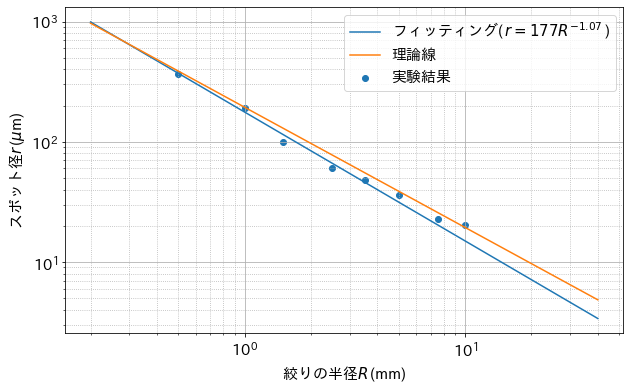
\includegraphics[width=13cm]{exp2_2.png}
    \caption{絞りの半径$R$とスポット径$r$の関係.理論値の$r$として第一暗点までの半径をとり,実験値の$r$としてスポットの半値全幅をとった.}
    \label{fig:exp2}
\end{figure}

\subsection{考察}
\subsubsection{アフォーカル光学系の設置}

\begin{figure}[htbp]
    \centering
    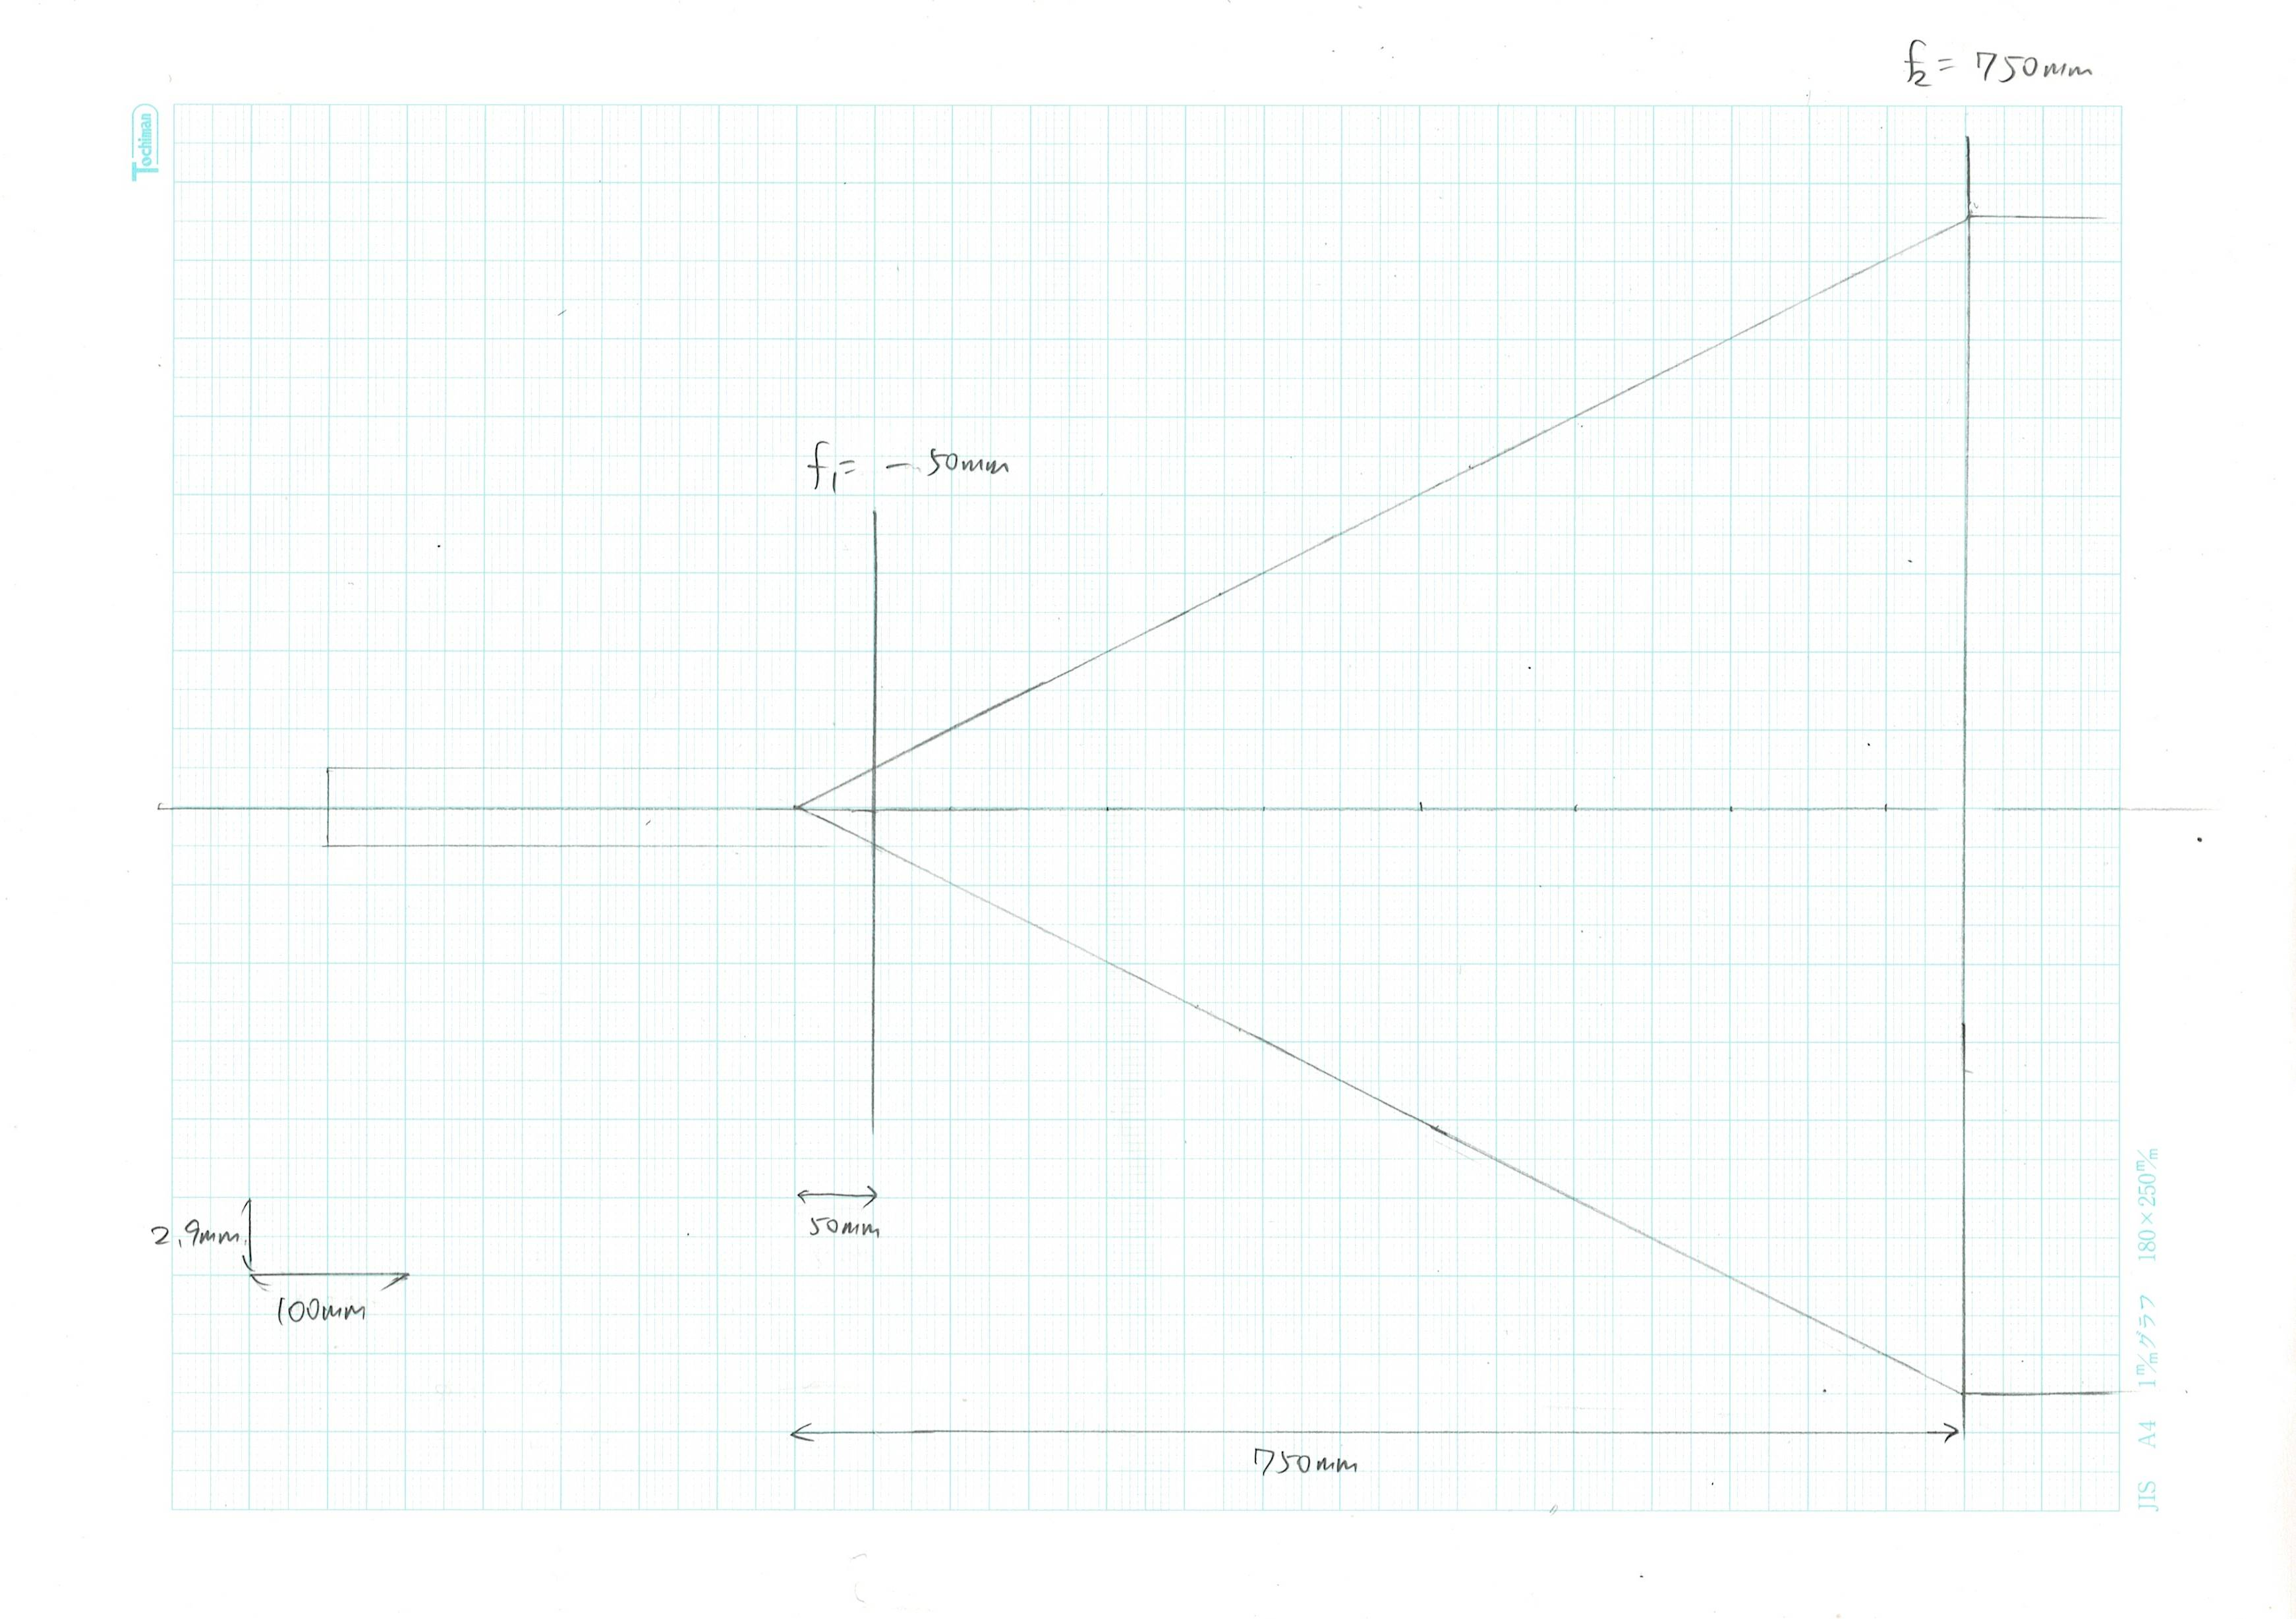
\includegraphics[width=15cm]{afforcal_fig.jpg}
    \caption{アフォーカル系の作図}
    \label{fig:afforcal}
\end{figure}

アフォーカル光学系によって拡大されたスポット径は,図\ref{fig:afforcal}上での三角形の相似から
\begin{equation}
    r_0 = \frac{750}{50} \times 2.9\,\mathrm{mm} = 43.5\,\mathrm{mm}
\end{equation}
と求まる.
得られた測定値35\,mmはここからかなりずれている.
これについては定規がスポットの中心からずれていたりスポットの縁の暗い部分を見逃していたりしたことで,測定値の方が小さくなったと考えられる.

\subsubsection{スポット径の計測}
絞りにより半径$R$となったレーザーを焦点距離$f$のレンズで集光し,カメラで集光点をカメラで撮影する場合,画像上に光軸を中心とする極座標$(\rho',\theta')$をとると式\eqref{bessel},式\eqref{limit}が成り立つ.
これをもとに絞りの半径$R$とスポット径$r$の関係を求めて図示すると図\ref{fig:exp2}のオレンジ色の直線になる.
また実験結果をフィッティングした結果$R\propto r^{-1.07}$と求まったので,理論式から予想される通りおおよそ$R \propto r^{-1}$となることが分かった.
実験結果と理論線のずれの原因としては,本来ベッセル関数に従う輝度分布をガウス分布で近似したことや,近似に用いた直線がスポットの中心からずれたことなどが考えられる.
事実フィッティングを確認すると,ガウス分布の半値全幅が実際のスポット径よりも小さく見積もられていることが読み取れる(図\ref{fig:fitr}).
そのためこうしたフィッティングの誤差を考えると,概ね実験結果は理論線に沿っているといえ,今回の実験系でスポット径は式\eqref{limit}に従う回折限界によって決まると結論できる.

\begin{figure}[htbp]
    \centering
    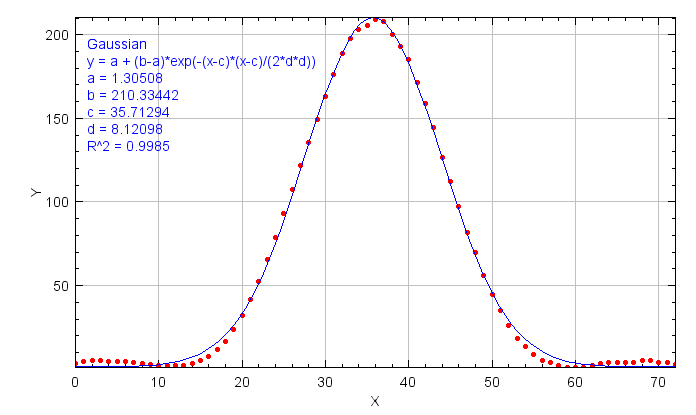
\includegraphics[width=13cm]{3mm.png}
    \caption{$2R=3$\,mmのときの輝度分布.ガウス分布の半値全幅の2倍($2r$)は約38\,pxと計算されたが,輝度分布から読み取れるスポットの直径は約45\,pxとやや大きい.他の$R$についても同様のことが分かった.}
    \label{fig:fitr}
\end{figure}

\section{実験3}
ここでは試料への照明の方法として,クリティカル照明・散光照明および(レンズ1枚を用いた)一様照明を実際に試し,それぞれの特徴を調べた.

\subsection{手法}
実験2で設置したレンズを取り外し,LED光源から400\,mmの位置に焦点距離200\,mmのレンズを置いた.
その後レンズの後方でスクリーンを動かし,光源の模様がはっきり見えるところでスクリーンを止めた(クリティカル照明).
またスクリーンをその位置からレンズの後方にある程度ずらした(散光照明).
最後にレンズを光源から200\,mmの位置に移動させ,スクリーンをレンズの後側焦点の位置に置いた(一様照明).
そしてこれらそれぞれの照明方法の特徴を観察した.

\subsection{結果}
クリティカル照明の場合,スクリーンに光源の模様がはっきりと見えた.
散光照明の場合,スクリーンには大きな円形のぼやけた像が見えた.
また散光照明と比べてクリティカル照明の方がスクリーンが明るかった.
一様照明の場合には照明のムラはなくなったが,スクリーンを後ろに動かすと照明は暗くなった.

\subsection{考察}

\begin{figure}[htbp]
    \centering
    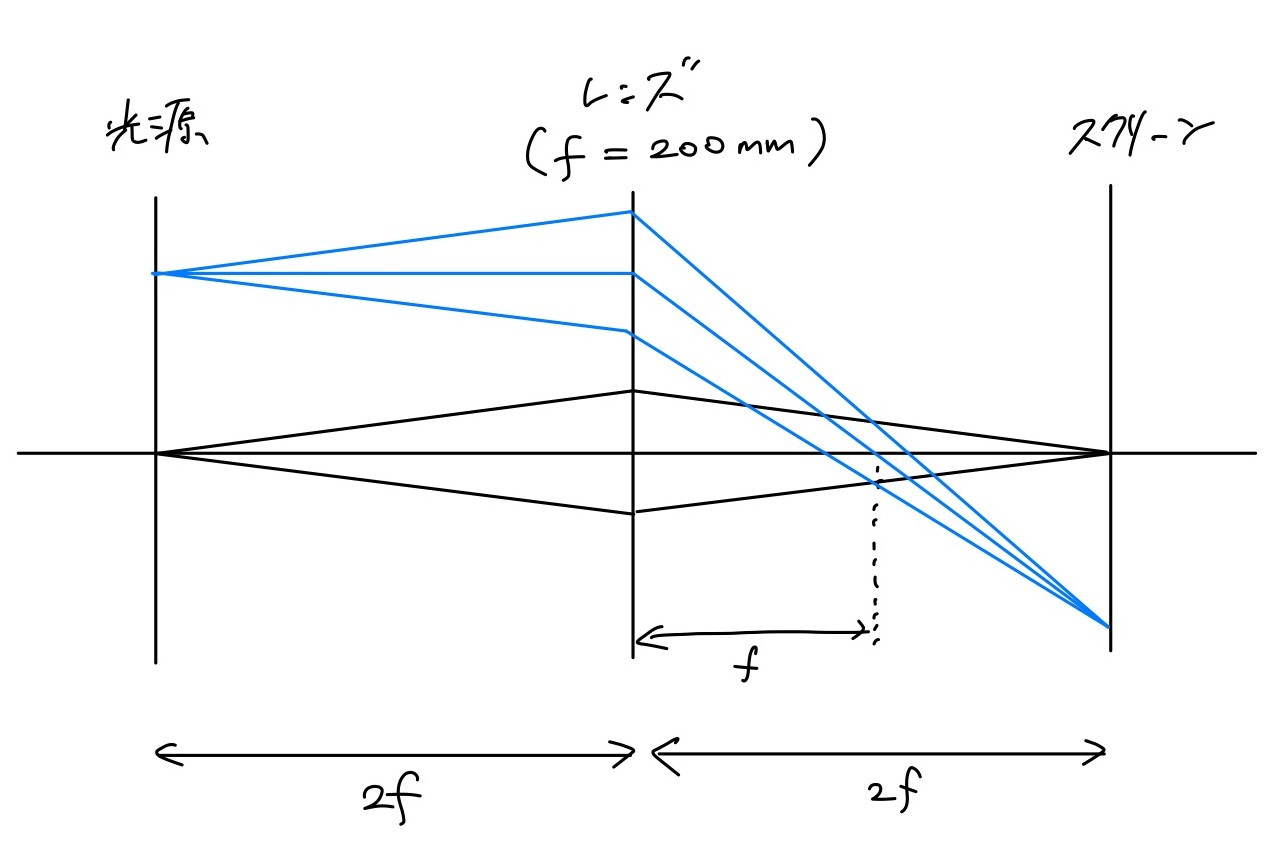
\includegraphics[width=10cm]{critical.jpg}
    \caption{クリティカル照明の作図}
    \label{fig:critical}
\end{figure}

\begin{figure}[htbp]
    \centering
    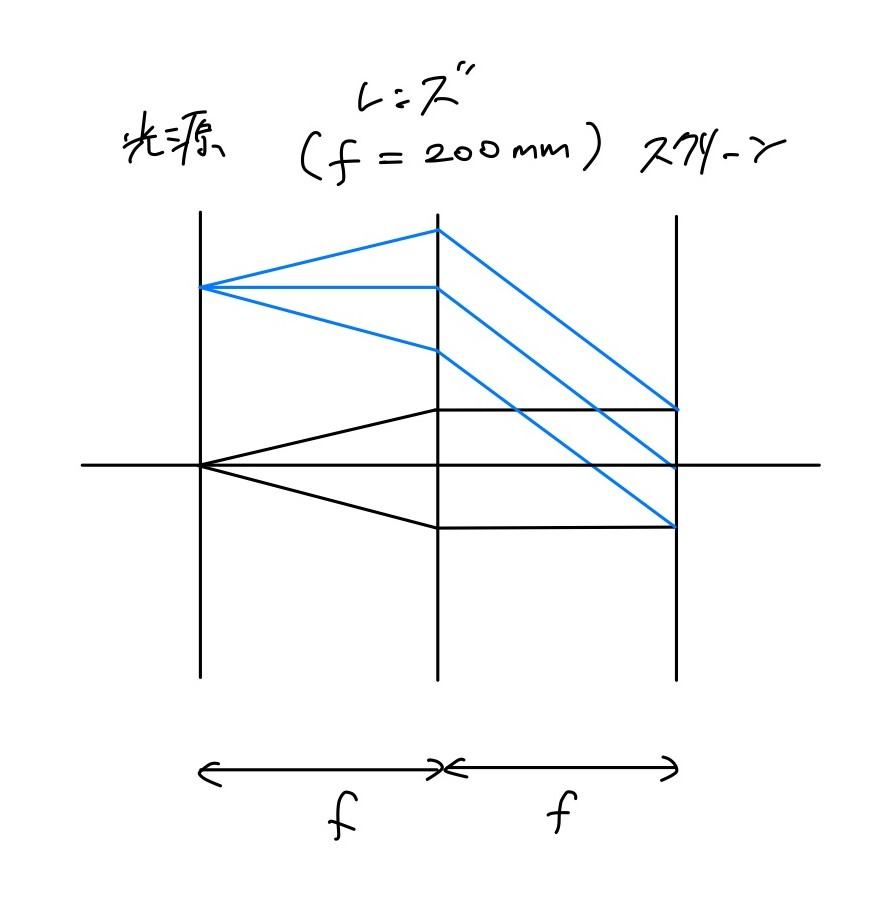
\includegraphics[width=10cm]{singlekohler.jpg}
    \caption{単一レンズを用いた一様照明の作図}
    \label{fig:singlekohler}
\end{figure}

今回の照明はいずれも光源とレンズの距離がレンズの焦点距離の2倍$2f$に等しい.
よってレンズの公式より,レンズ後方に$2f$だけ進んだ位置に像ができる.
スクリーンがちょうどこの位置にあるのがクリティカル照明であり,光がスクリーン上で光軸付近に集中して明るく照らされる(図\ref{fig:critical}).
しかし光源のむらもそのまま投影されるため,光源の情報がスクリーンに加わってしまう.
一方でそこからスクリーンを後方にずらしたものが散光照明である.
この場合後方にずらせばずらすほど光はスクリーン上でぼやけて照明は一様に近づく.
しかし同時に光が分散することで照明は暗くなってしまう.
またレンズを移動させて一様照明をしたときの作図が図\ref{fig:singlekohler}である.
作図から,光源のすべての点から出た光がスクリーン上で平行光として一様に照射されることが分かるので,光源の情報は慣らされて一様な照明が実現すると考える.
ただしスクリーンを後方に下げると,光源の光軸から離れた位置由来の光がスクリーンの外側に広がってしまう.
これがスクリーンを後ろに動かしたときに照明が暗くなった理由と考える.

\section{実験4}
実験3に引き続き,試料を一様にかつ明るく照明する方法であるケーラー照明を試し,その特徴を調べた.

\subsection{手法}

\begin{figure}
    \centering
    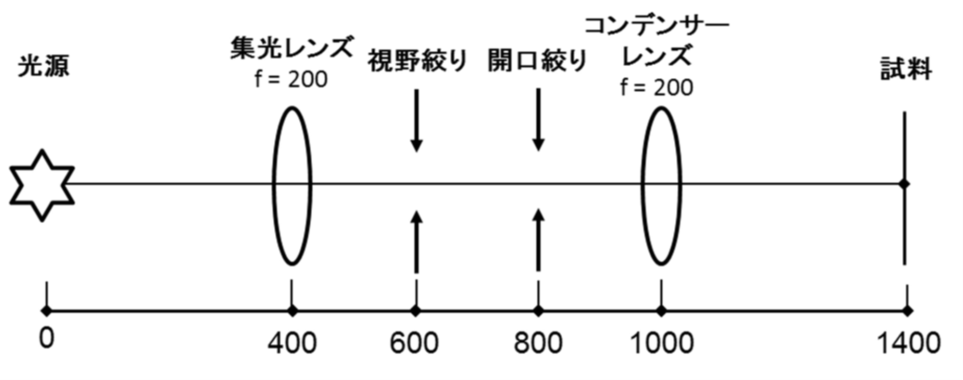
\includegraphics[width=13cm]{kohler.png}
    \caption{ケーラー照明.実験4では「試料」とあるところにスクリーンを置いた.}
    \label{fig:kohler}
\end{figure}

図\ref{fig:kohler}のように集光レンズ(焦点距離200\,mm),視野絞り,開口絞り,コンデンサーレンズ(焦点距離200\,mm),スクリーンを置いた(ケーラー照明).
まず視野絞りの直径を15\,mmに設定して2つめの絞りをできるだけ閉じ,開口絞りの上に光源の像ができていることを確認した.
次に開口絞りをわずかに開けてスクリーンを前後させることで,コンデンサーレンズから出た光が平行光であることを確認した.
最後にスクリーンの位置をもとに戻し,開口絞りを開けて視野絞りを半分程度閉じた.
このとき視野絞りの像がスクリーンに投影されていることを確認した.

\subsection{結果}
どれも確認できた.

\subsection{考察}

\begin{figure}[htbp]
    \centering
    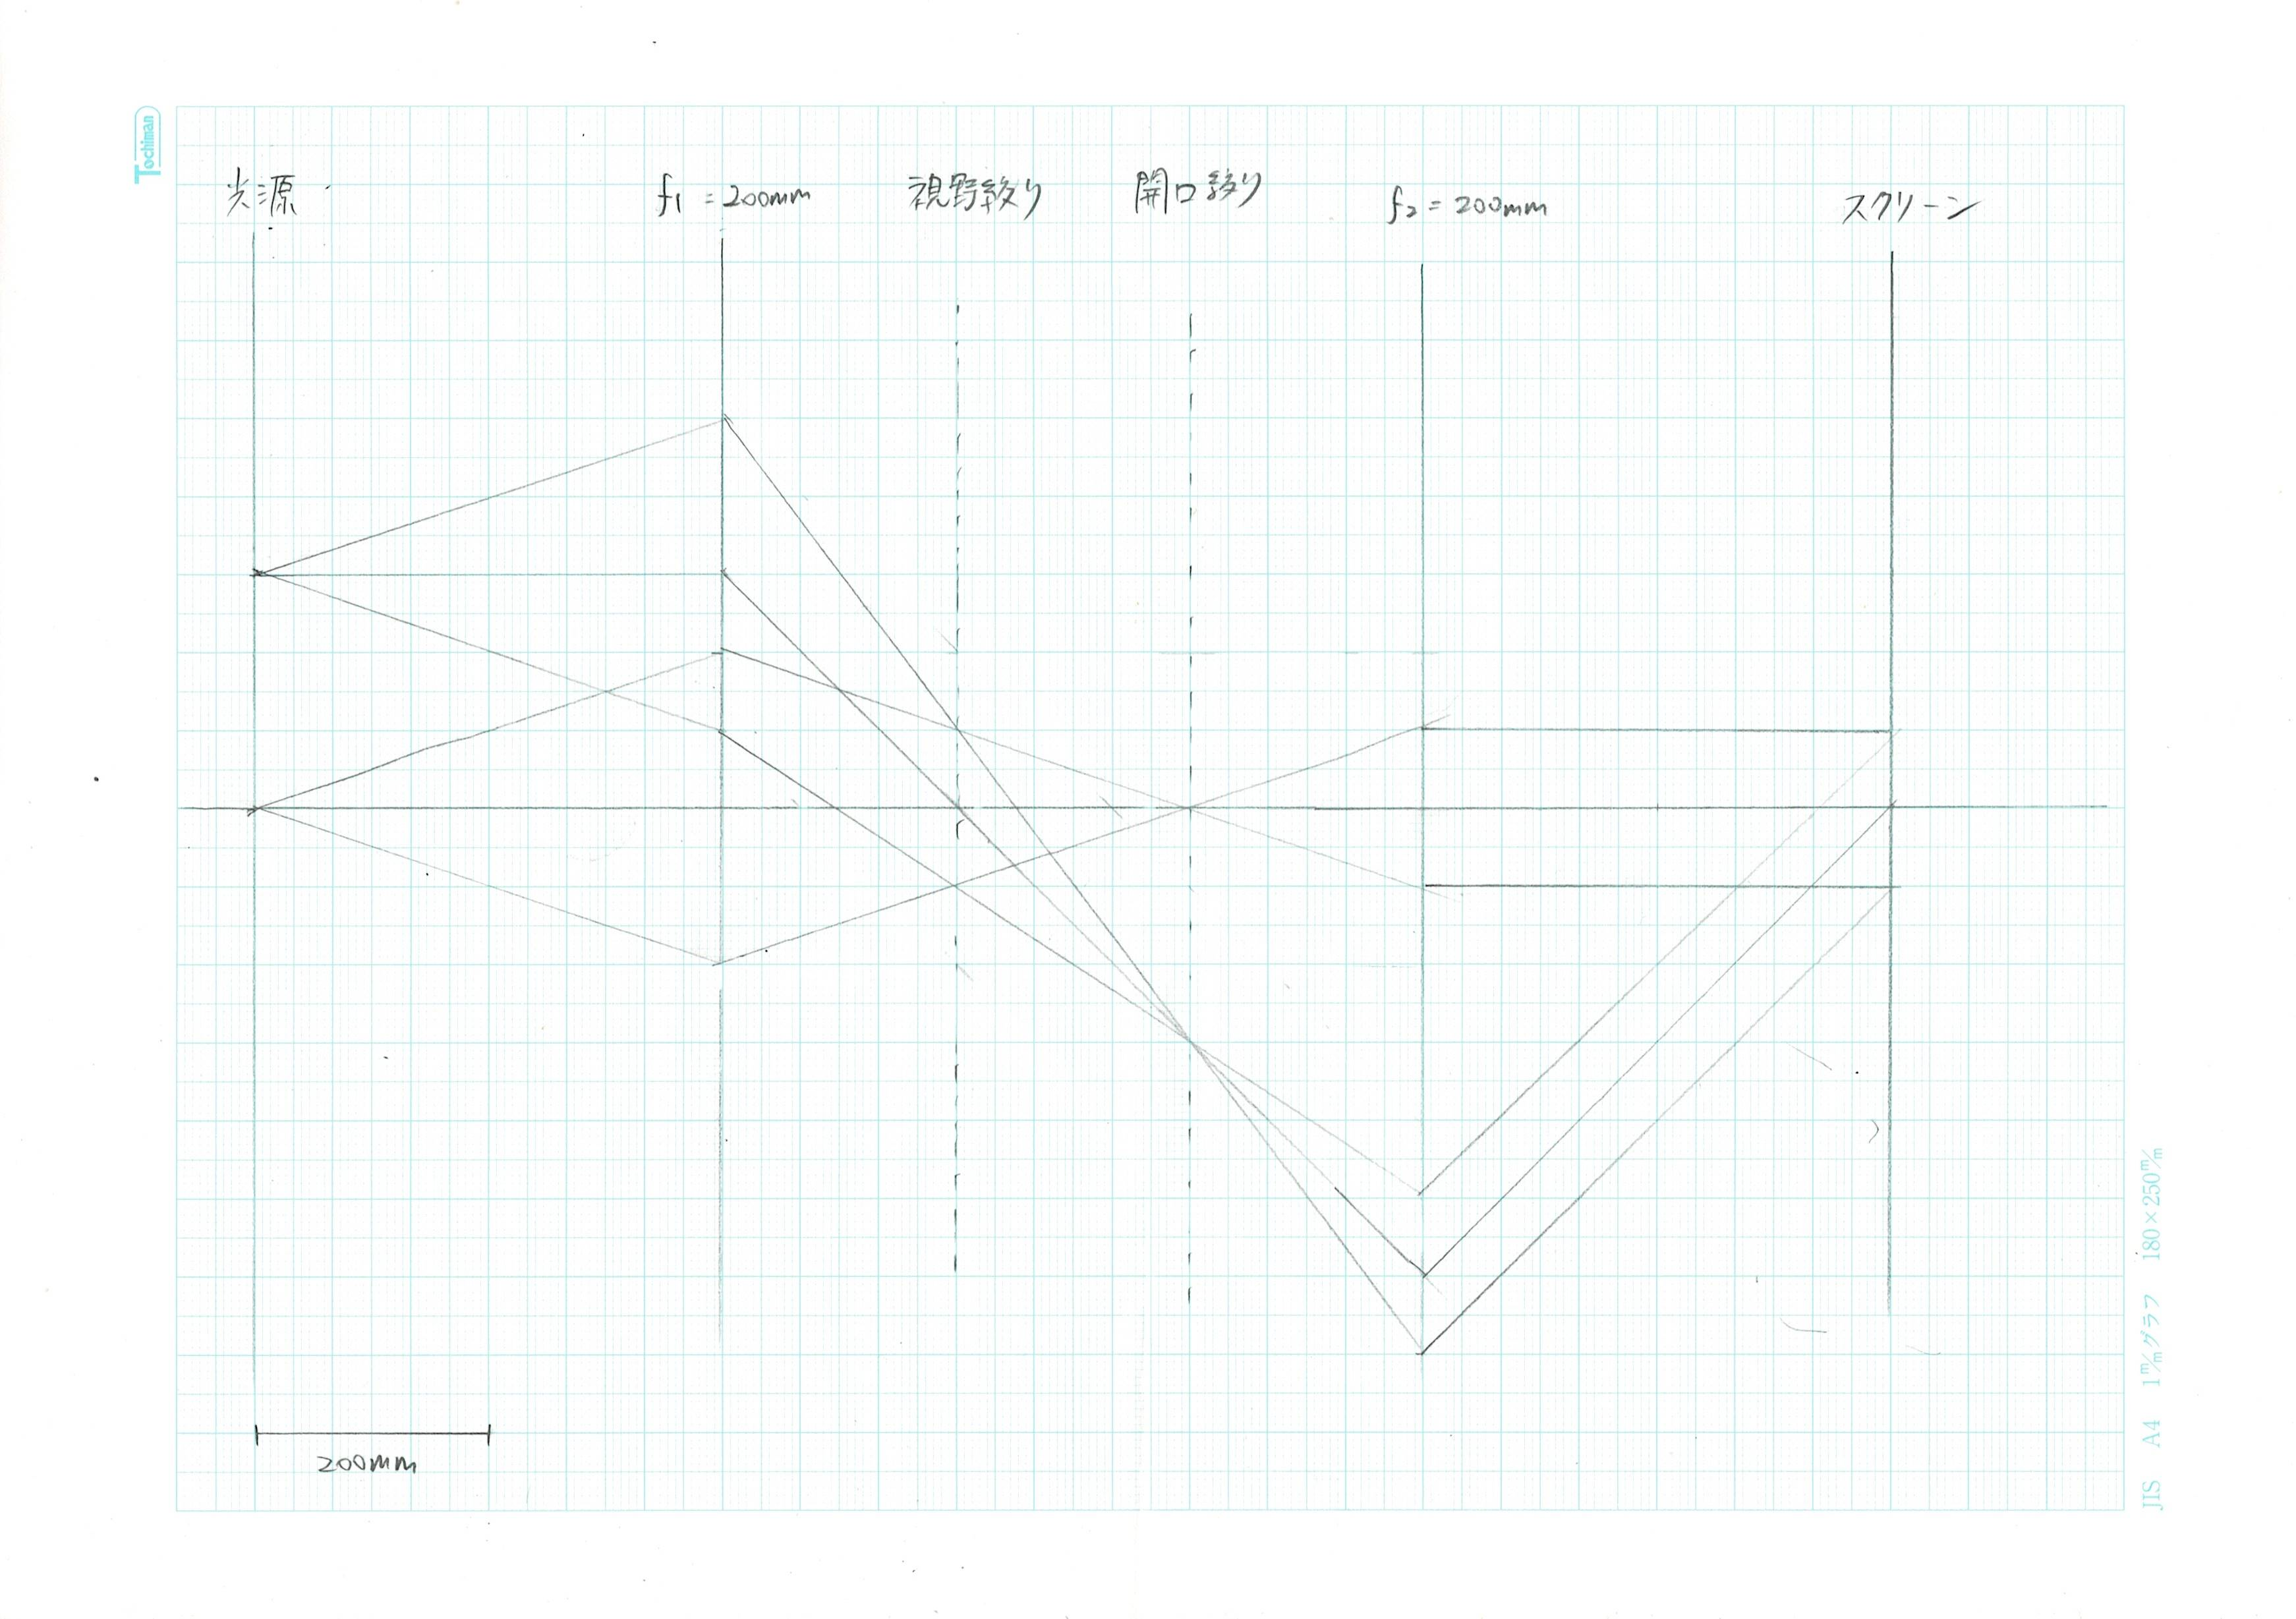
\includegraphics[width=15cm]{kohler_fig.jpg}
    \caption{ケーラー照明の作図}
    \label{fig:kohler_fig}
\end{figure}

ケーラー照明の作図を行うと図\ref{fig:kohler_fig}のようになる.
これより光源の像が開口絞りの上に結ばれることと,視野絞りの像がスクリーンに結ばれることが分かる.
(このことは実験で確認できた.)
よって光源と開口絞りは共役な位置にあり,視野絞りはスクリーンと共役な位置にある.
そのため開口絞りを閉じることは光源の範囲を狭めることと同義であり,このときスクリーンに到達する光の量が減るため照明は暗くなる.
後に説明するように照明は一様なので,このときも照明全体が一様に暗くなる.
また開口絞りを閉じると光源の光軸から離れた場所からの光が届かなくなり,スクリーンに照射される光の光軸に対する傾き$\theta$は小さくなる.
すなわち開口数$n\sin{\theta}$($n$は媒質の屈折率.今回は空気なので$n=1$)が小さくなる.
これが開口絞りの名前の由来であると考える.

一方視野絞りを閉じることはスクリーン上の像の範囲が狭まることと同義であり,そのためにスクリーン上の照明される場所は狭くなる.
ただし開口絞りを操作しない限り照明の明るさは変わらない.
そのためスクリーンの位置に試料があるとき,視野絞りを閉じると試料が明るく見える範囲(観察者にとっての「視野」)が狭まることになる.
これが視野絞りの名前の由来であると考える.

最後に,ケーラー照明で一様な照明が実現する理由を説明する.
図\ref{fig:kohler_fig}に示した通り,光源のどの点から出た光も最終的に平行光となってスクリーンのある共通の場所を照らす.
そのため光源にムラがあってもスクリーンに現れる照明は一様となる.

\section{実験5}
ここではケーラー照明で試料を照らし,試料の像をカメラに映す光学系(顕微鏡の光学系)を作成した.

\subsection{手法}

\begin{figure}
    \centering
    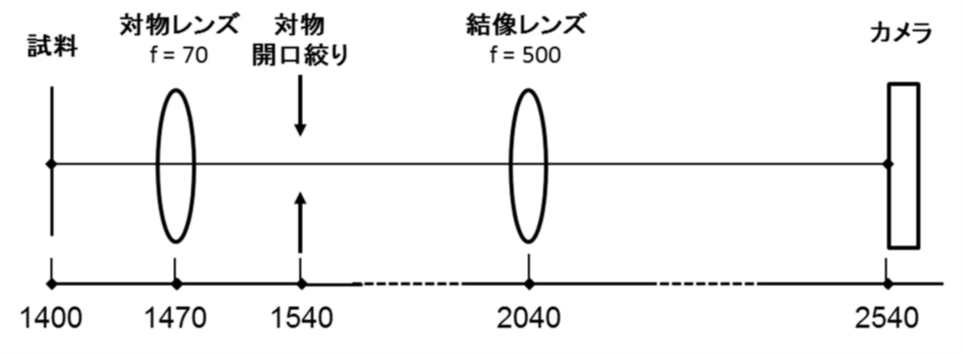
\includegraphics[width=13cm]{obj.png}
    \caption{観察系の結像光学系}
    \label{fig:obj}
\end{figure}

実験4のケーラー照明のスクリーンの代わりに試料を置いた.
そしてその後方に対物レンズ(焦点距離70\,mm),対物開口絞り,結像レンズ(焦点距離500\,mm)を図\ref{fig:obj}のように並べた光学系を組んだ.
また試料ホルダに20\,$\mu$m,100\,$\mu$m間隔の格子縞の試料を入れ,カメラでその像を撮影した.
(試料の位置をずらすことでカメラに映す格子縞を切り替えることができる.)
次にカメラに映す格子縞を20\,$\mu$mにしてから650\,nmのカラーフィルタを視野絞りの直後に入れて再び撮影した.
その後試料位置を調整してフォーカスを合わせて撮影し直した.
その後カラーフィルタを450\,nmのものに取り替えて再び同様の撮影を行った.
またカメラに映す格子縞を100\,$\mu$mにして再び同じ撮影を行った.
ただし650\,nmのカラーフィルタの撮影は省略した.

次に照明側の視野絞り,開口絞り(コンデンサー絞り),観察側の開口絞り(対物絞り)をそれぞれをそれぞれ開閉し,カメラに映る像の変化を観察・撮影した.

最後にImageJを用いて画像上での格子縞の大きさをもとの格子縞の大きさと比較して,この顕微鏡光学系の倍率を算出した.

\subsection{結果}

\begin{figure}[htbp]
    \centering
    \begin{subfigure}{0.3\columnwidth}
        \centering
        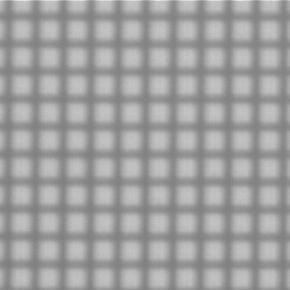
\includegraphics[width=\columnwidth]{20um_white_tri.png}
        \caption{カラーフィルタなし}
        \label{fig:20white}
    \end{subfigure}
    \begin{subfigure}{0.3\columnwidth}
        \centering
        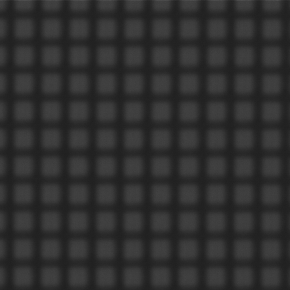
\includegraphics[width=\columnwidth]{20um_red2_tri.png}
        \caption{カラーフィルタ(650\,nm)あり}
        \label{fig:20red}
    \end{subfigure}
    \begin{subfigure}{0.3\columnwidth}
        \centering
        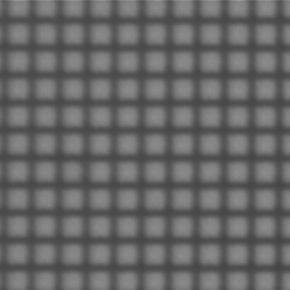
\includegraphics[width=\columnwidth]{20um_blue2_tri.png}
        \caption{カラーフィルタ(450\,nm)あり}
        \label{fig:20blue}
    \end{subfigure}    
    \caption{20\,$\mu$mの格子縞を撮影した画像(カラーフィルタを入れたときの画像はフォーカスを合わせた後のもの)}
    \label{fig:20}
\end{figure}

\begin{figure}[htbp]
    \centering
    \begin{subfigure}{0.4\columnwidth}
        \centering
        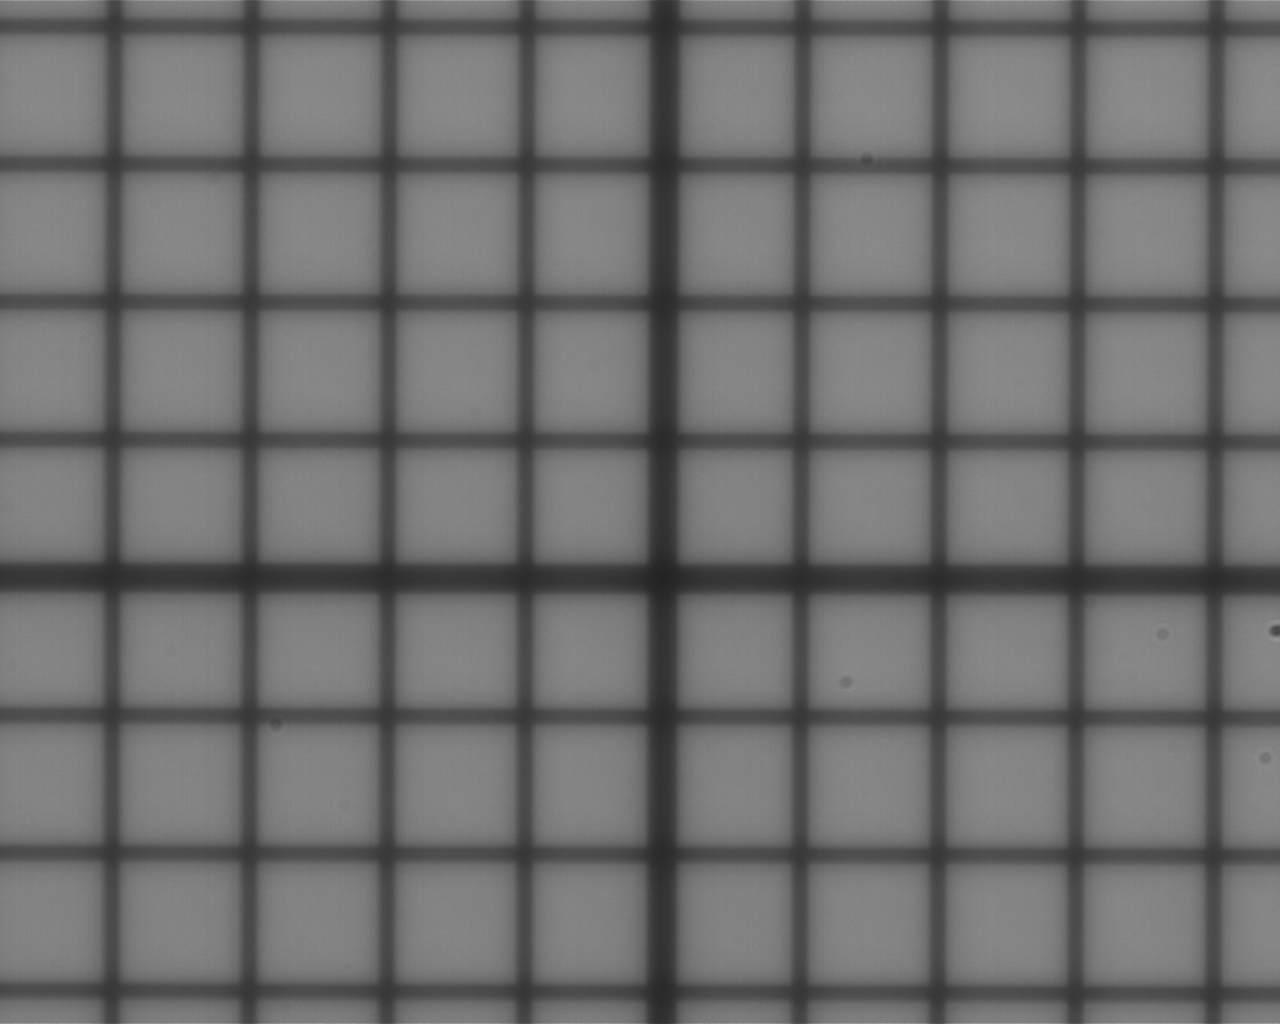
\includegraphics[width=\columnwidth]{100um_white.png}
        \caption{カラーフィルタなし}
        \label{fig:100white}
    \end{subfigure}
    \begin{subfigure}{0.4\columnwidth}
        \centering
        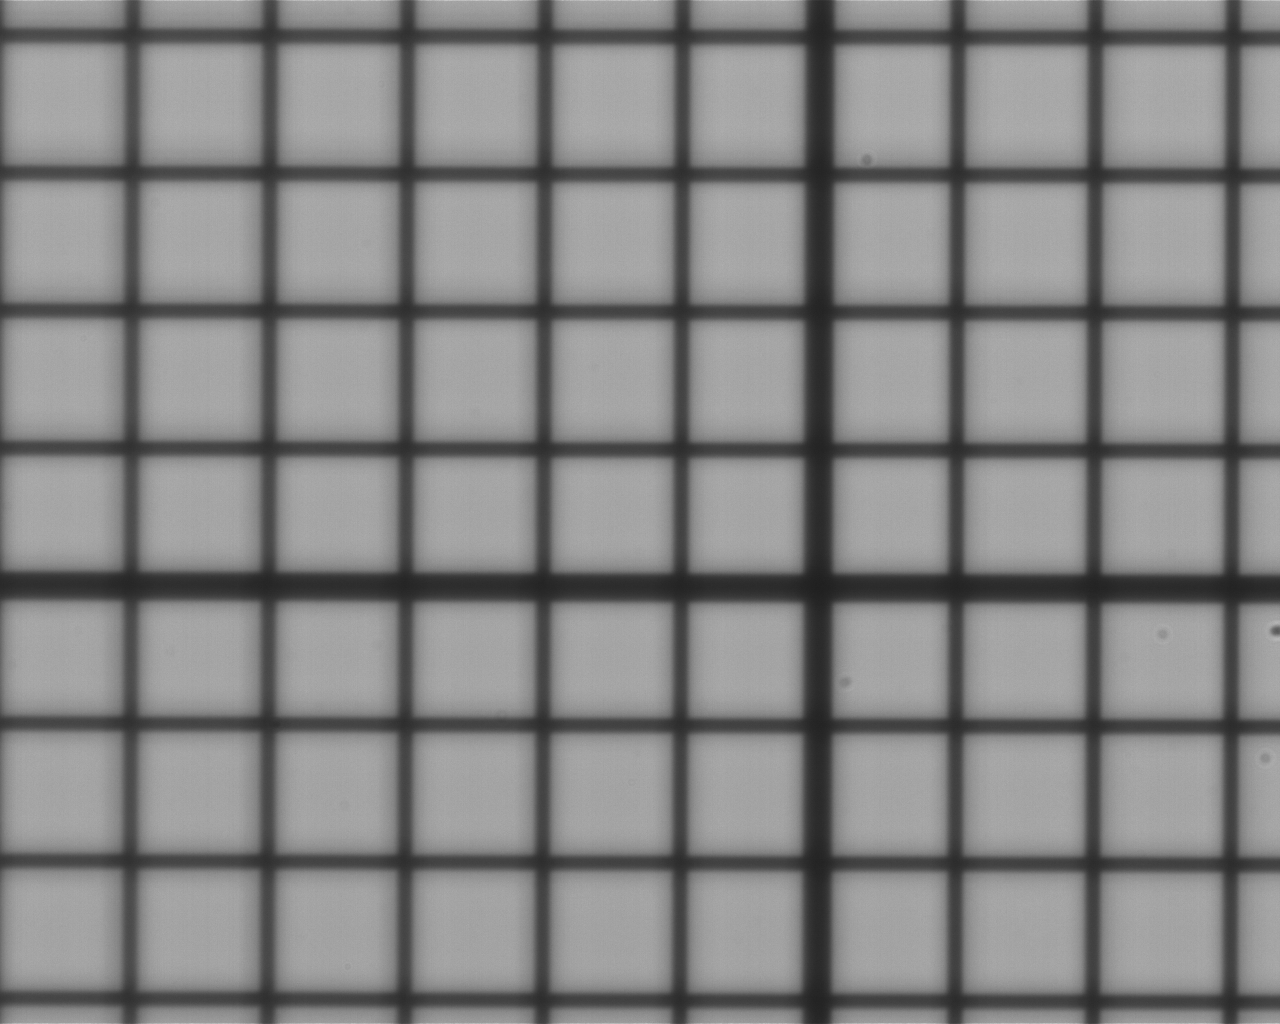
\includegraphics[width=\columnwidth]{100um_blue.png}
        \caption{カラーフィルタ(450\,nm)あり}
        \label{fig:100blue}
    \end{subfigure}    
    \caption{100\,$\mu$mの格子縞を撮影した画像(カラーフィルタを入れたときの画像はフォーカスを合わせた後のもの)}
    \label{fig:100}
\end{figure}

\begin{figure}[htbp]
    \centering
    \begin{subfigure}{0.3\columnwidth}
        \centering
        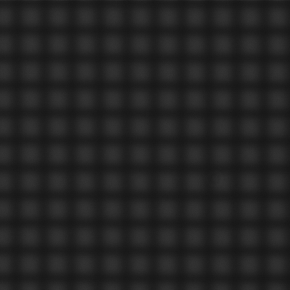
\includegraphics[width=\columnwidth]{20um_blue_obj5mm_tri.png}
        \caption{対物絞り5\,mm}
        \label{fig:obj5}
    \end{subfigure}
    \begin{subfigure}{0.3\columnwidth}
        \centering
        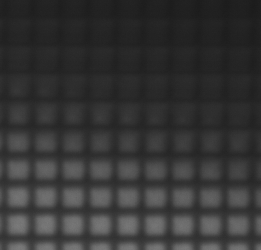
\includegraphics[width=\columnwidth]{20um_blue_shiya_tri.png}
        \caption{視野絞り}
        \label{fig:shiya}
    \end{subfigure}
    \begin{subfigure}{0.3\columnwidth}
        \centering
        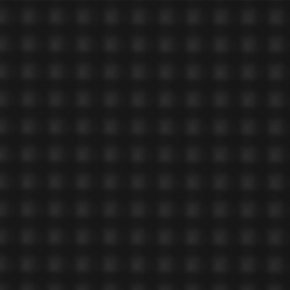
\includegraphics[width=\columnwidth]{20um_blue_condensor10mm_tri.png}
        \caption{コンデンサー絞り10\,mm}
        \label{fig:cond10}
    \end{subfigure}    
    \caption{各々の絞りをある程度閉じて20\,$\mu$mの格子縞を撮影した画像}
    \label{fig:20_sibori}
\end{figure}


まず20\,$\mu$mの格子縞を撮影した結果が図\ref{fig:20}である.
図\ref{fig:20white}はカラーフィルタを置かずに撮影したものであり,図\ref{fig:20red}は650\,nmのカラーフィルタを,図\ref{fig:20blue}は450\,nmのカラーフィルタを通して撮影したものである.
また同様の撮影を100\,$\mu$mの格子縞について行った結果が図\ref{fig:100}である.
ただしカラーフィルタを置いた後そのまま撮影した画像はどれもフォーカスが合っていなかったので,フォーカスを調整したものをここに載せた.
これらの画像から,カラーフィルタを入れることでコントラストが強まったことが分かる.

次に20\,$\mu$mの格子縞に切り替えて,光学系のそれぞれの絞りを閉じて撮影した結果が図\ref{fig:20_sibori}である.
対物絞りを閉じると全体が一様に暗くなって格子縞の像がぼやけたことが分かる(図\ref{fig:obj5}).
また視野絞りを閉じると画像の一部が暗くなり,それ以外の部分はコントラストが少し強まった(格子の縁の色が若干濃くなった)ことが確認できる(図\ref{fig:shiya}).
そしてコンデンサー絞りを閉じると全体が一様に暗くぼんやりとしたことが確認できる(図\ref{fig:cond10}),

最後に100\,$\mu$mの格子縞が図\ref{fig:100blue}上では約137\,pxの格子縞となっていた.
カメラの1\,pxが5.2\,$\mu$mに対応することから,倍率は7.12倍と計算できる.

\subsection{考察}
まずカラーフィルタを入れることで画像のコントラストが強まったのは,色収差がなくなったためと考えられる.
白色のLED光源は様々な波長の光が重ね合わさっており,それらはレンズを通したときに異なる角度で屈折する.
そのためある波長で結像が起こっても他の波長では結像が起こらず,像はぼやけることになる(色収差).
しかし特定の波長だけ通すカラーフィルタを入れることですべての光がほぼ同じ角度に屈折し,像のぼやけが解消される.
実験ではこれによってコントラストが強まったと考えられる.
また実験ではカラーフィルタを入れた直後はフォーカスが合っていなかったが,これは波長によって屈折率が異なるというこの説明を裏付けている.

\begin{figure}[htbp]
  \centering
  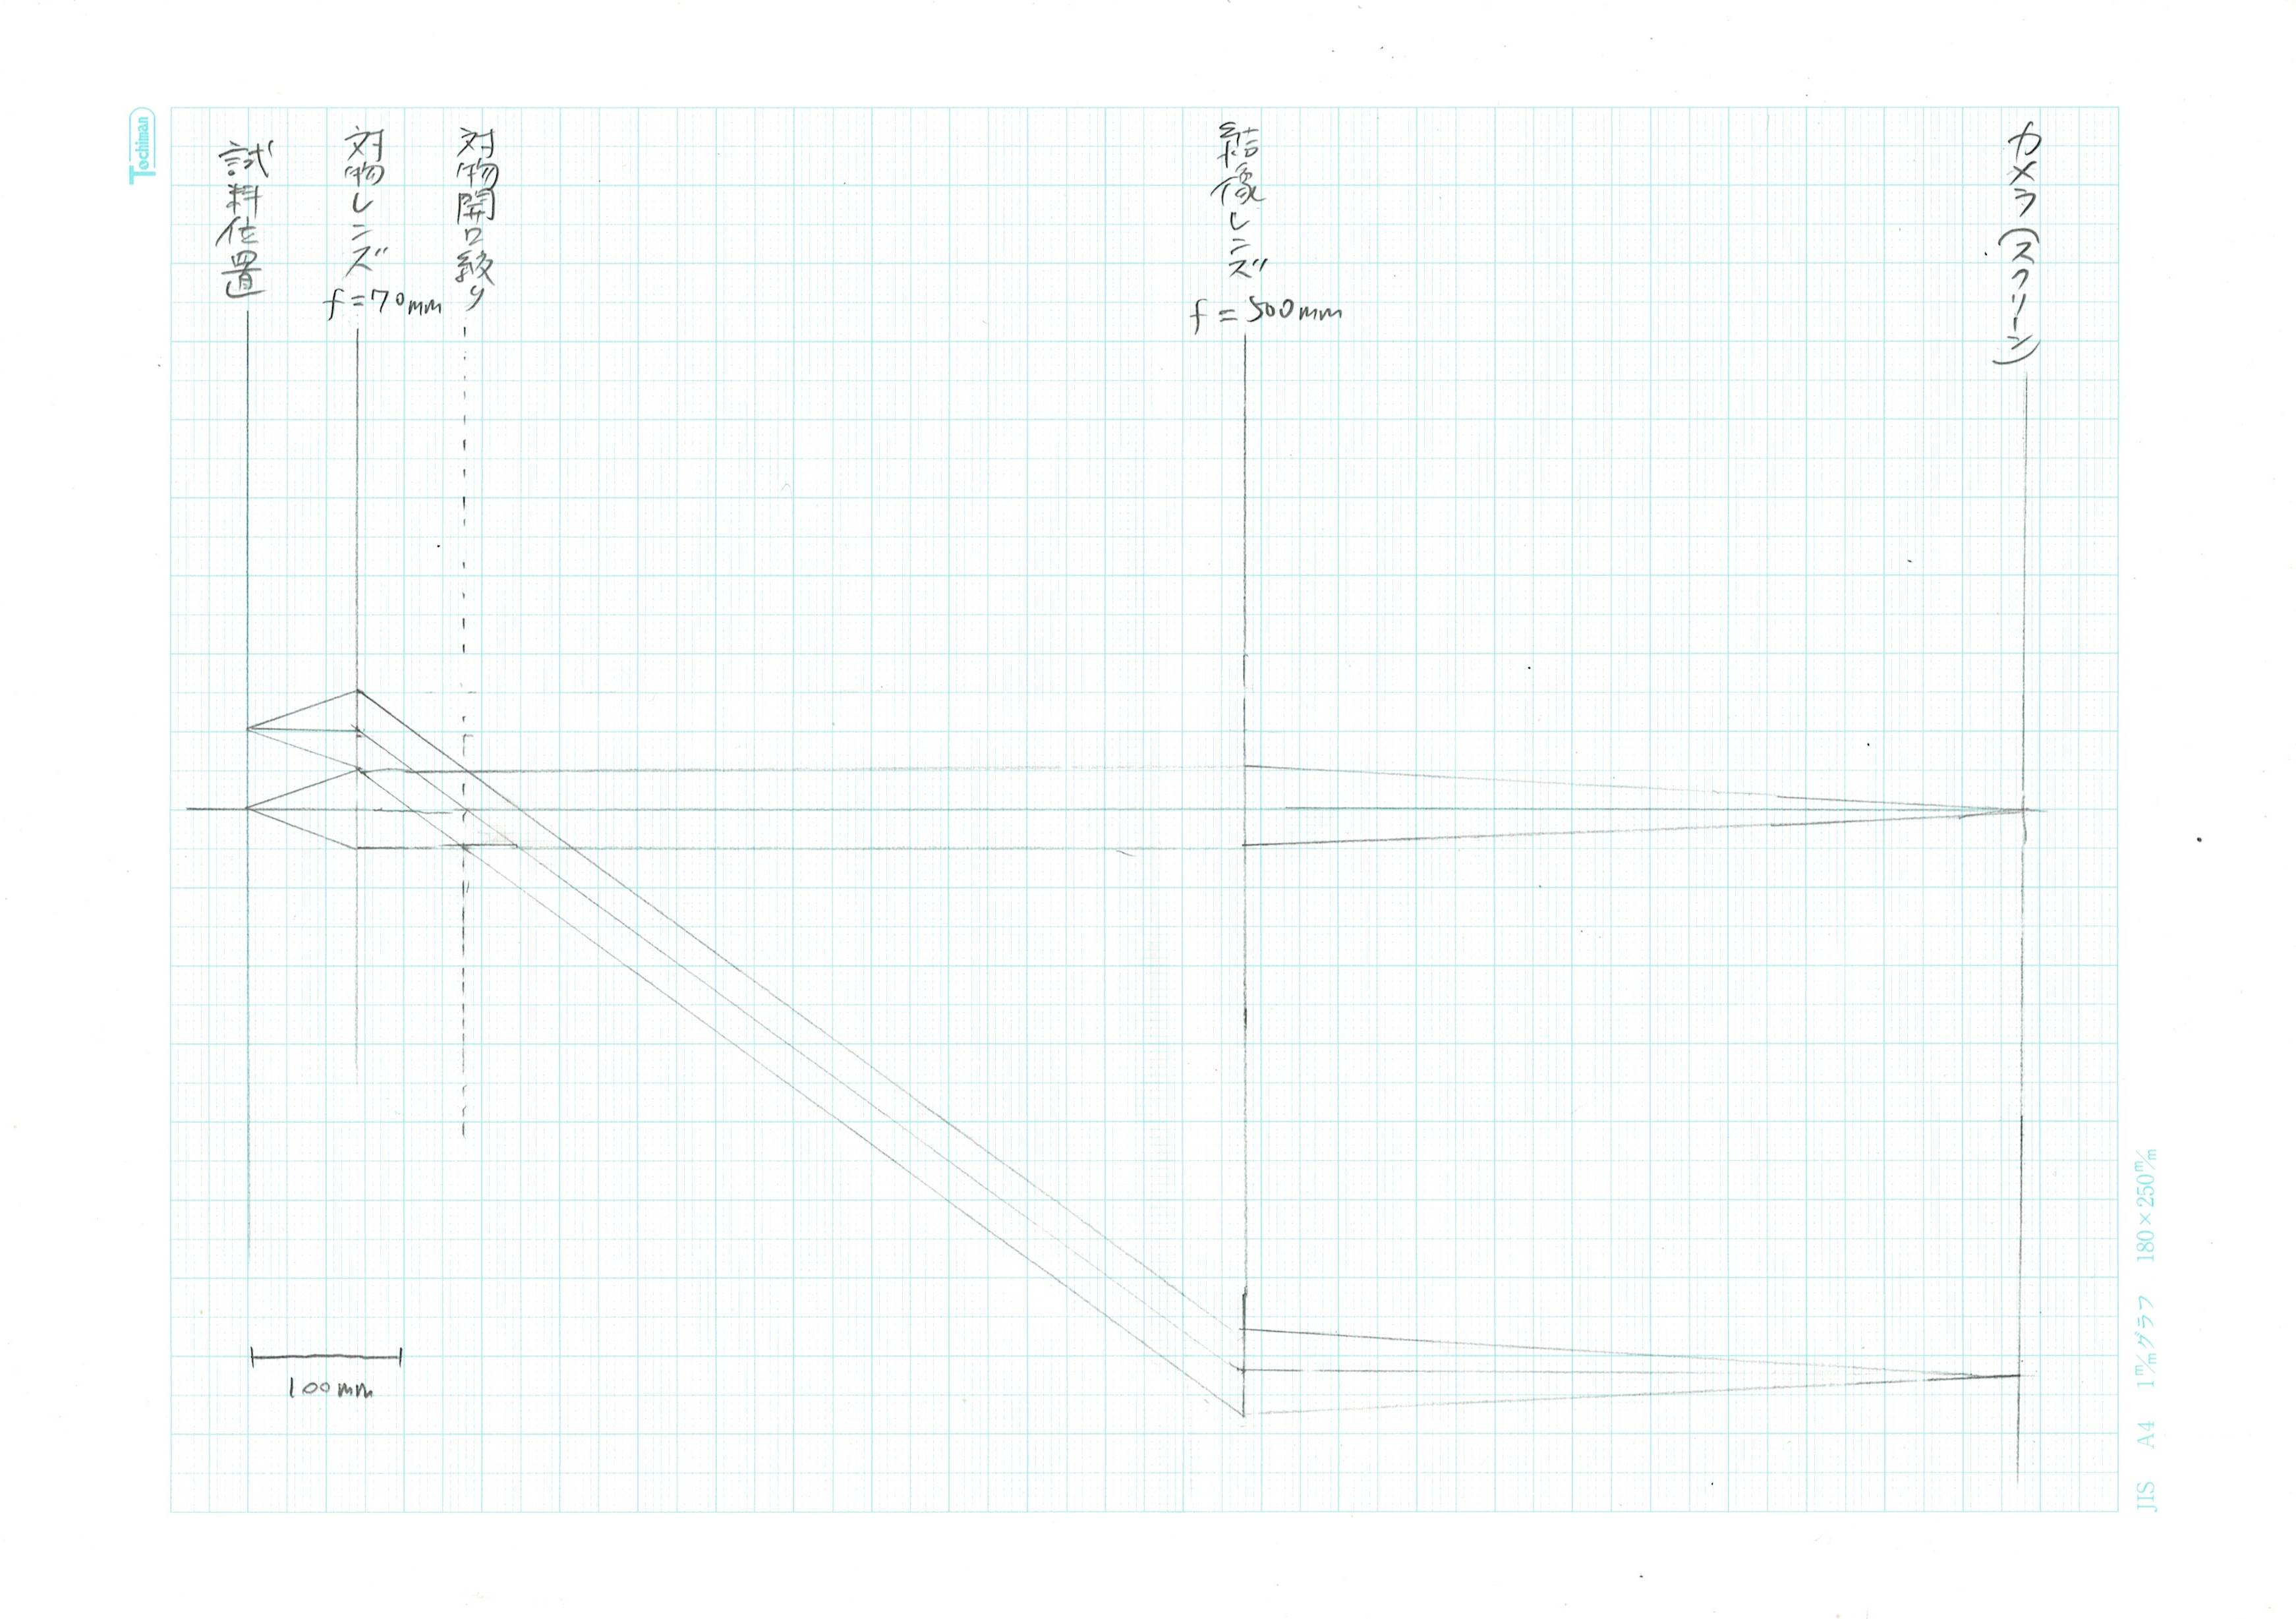
\includegraphics[width=15cm]{obj_fig.jpg}
  \caption{観察系の作図}
  \label{fig:obj_fig}
\end{figure}

次に絞りを閉じた場合の画像の変化を考察する.
対物絞りを閉じた場合は実験6の考察で後述するようにもとの画像の高周波成分をカットした状況に相当する.
そのため全体的に滑らかになり格子縞の像がぼやけたと考えられる.
また画像が全体的に暗いのは,絞りを閉じたことでカメラに達する照明光の量が減少したからと考えられる.

まず視野絞りを閉じた場合を考える.
このとき実験4で考察したとおり照明の明るさは変わらずにその範囲が狭まる.
そのため画像上では絞りを閉じる前と変わらない部分と暗くなる部分に分かれる.
またコントラストが強まった理由は,視野絞りを閉じることで光軸から離れた光が遮られ,ホルダーのエッジ部分での乱反射などに由来する迷光の寄与を抑えられたからと考えられる.

コンデンサー絞りを閉じた場合は照明が一様に暗くなる.
そのため得られる画像ももとより暗くなるが,対物絞りを閉じたときとは異なり試料の情報が書き換わることはないと考えられる.

\section{実験6}
ここでは対物レンズによって試料の像を瞳面に投影し,それが試料により生じた明暗のパターンのフーリエ変換になっていることを確認した.

\subsection{原理}

\begin{figure}[htbp]
    \centering
    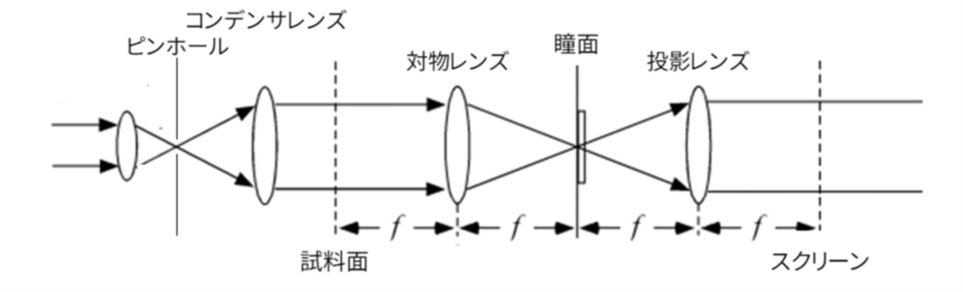
\includegraphics[width=14cm]{4fsystem.png}
    \caption{4f光学系}
    \label{fig:4fsystem}
\end{figure}

図のような対物レンズと投影レンズ(結像レンズ)の焦点距離の等しい4f光学系を考える.
実験2の原理で述べた通り,レンズから焦点距離だけ離れた所における像はレンズの位置の像のフーリエ変換となる.
よってこの系では瞳面(実験では対物絞りの置かれている位置)に試料のパターンをフーリエ変換した像ができる.
さらにスクリーン(実験ではカメラの置かれている位置)に瞳面の像をフーリエ変換した像ができる.
つまりスクリーンには試料を二度フーリエ変換した像が投影される.

ここでは1次元系を考え試料面に
\begin{equation}
    f(x) = 1 + \cos \left(2\pi \frac{x}{d}\right)
\end{equation}
というパターンがある場合を考える.
このとき式\eqref{foulier}を用いると瞳面の像のパターンは
\begin{equation}
    u(x') = A'_0 \int f(x) \exp \left(-\frac{kxx'}{f}\right) dx = A'_0 \left[ \delta \left(\frac{x'}{\lambda f}\right) +\frac{1}{2} \delta \left(\frac{x'}{\lambda f} - \frac{1}{d} \right) + \frac{1}{2} \delta \left(\frac{x'}{\lambda f} + \frac{1}{d}\right) \right]
    \label{hitomi}
\end{equation}
と求まる.
ここで$\lambda$は光の波長であり,式$k = 2\pi / \lambda$を満たすことを用いた.
これより瞳面には
\begin{equation}
    x' = 0, \pm \lambda \frac{f}{d} \label{spot}
\end{equation}
の位置にスポットを持つ像が投影されることが分かる.
一方でスクリーンにはこれをさらにフーリエ変換したパターンが投影される.
しかし式\eqref{hitomi}の第1項をフーリエ変換しても定数にしかならないので,正弦波の情報を持つのは第2,3項である.
加えて瞳面で試料からの光が到達する範囲は対物レンズの半径を$r$として$-r<x'<r$に限られる.
よって試料の情報がスクリーンに現れる条件は
\begin{equation}
    \frac{\lambda f}{d} < r 
\end{equation}
である.
実験系で言い換えると対物絞りを半径$r$まで閉じたときの顕微鏡の分解能の限界は
\begin{equation}
    d = \frac{\lambda f}{r}
\end{equation}
で与えられる.

\subsection{手法}
実験5の光学系を引き続き用いた.
まずコンデンサー絞りをできるだけ絞りカメラの露光時間を1\,ms以下にしてから,対物絞りを外してカメラを対物絞りの位置に移動させた.
カメラを前後させて像が鮮明になる位置に調整し,20\,$\mu$mおよび100\,$\mu$mの間隔の格子縞の回折像をそれぞれ撮影した.

再びカメラをもとの位置に戻し,コンデンサ-絞りとカメラの露光時間を調整し,試料が映るようにした.
その後対物絞りがあった位置に空間フィルタ(縦スリット・横スリット)をセットしてから20$\mu$m間隔の格子縞を撮影した.
一方で実験5で撮影した20\,$\mu$m間隔の格子縞の画像(図\ref{fig:20blue})をフーリエ変換した画像を生成し,これと今回の実験結果を比較した.
フーリエ変換にはImageJのフーリエ変換機能を用いた.
またImageJ上でこのフーリエ変換した画像に空間フィルタを施してから再度フーリエ変換した画像を生成し,これと今回の実験結果を比較した.

\subsection{結果}
\begin{figure}[htbp]
    \centering
    \begin{subfigure}{0.4\columnwidth}
        \centering
        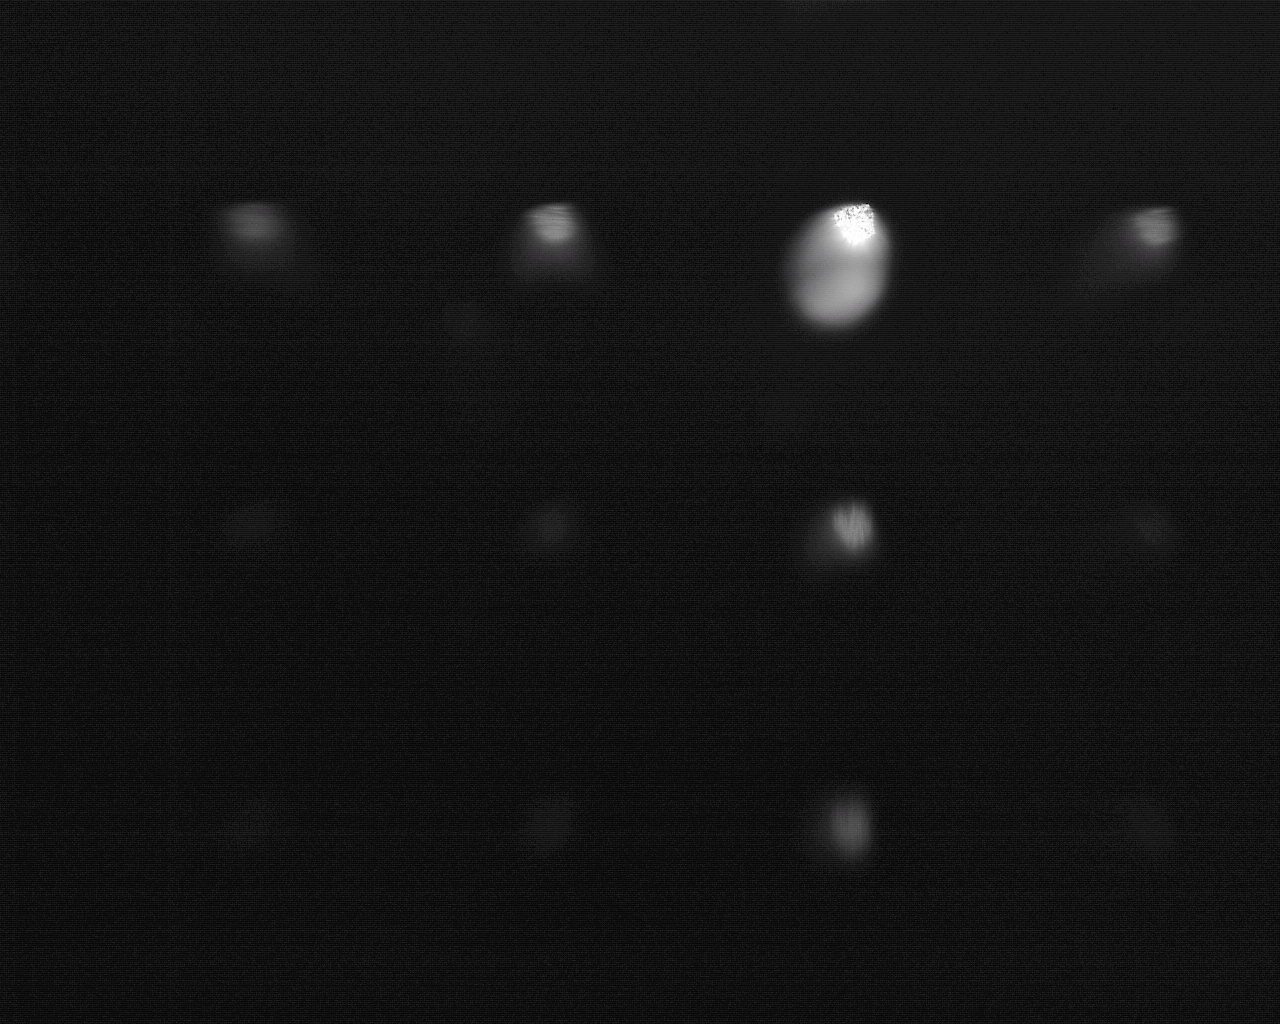
\includegraphics[width=\columnwidth]{20um_fourier_edit.png}
        \caption{20\,$\mu$m間隔}
        \label{fig:20fourier}
    \end{subfigure}
    \begin{subfigure}{0.4\columnwidth}
        \centering
        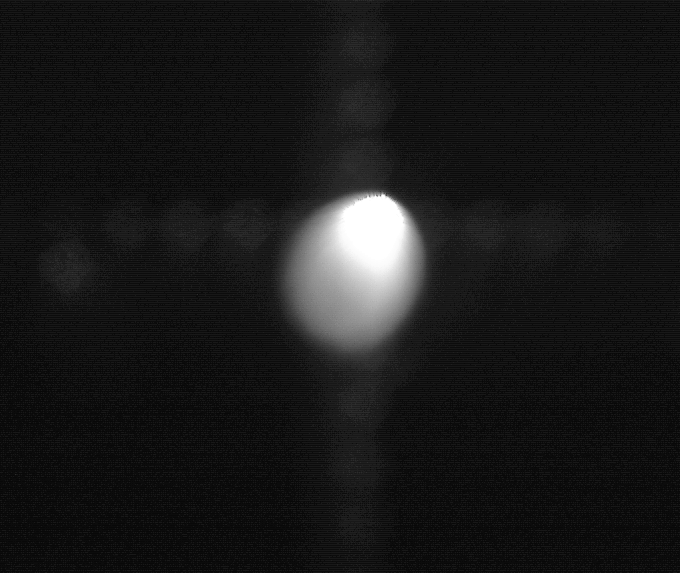
\includegraphics[width=\columnwidth]{100um_fourier_edit.png}
        \caption{100\,$\mu$m間隔}
        \label{fig:100fourier}
    \end{subfigure}    
    \caption{格子縞の回折像(スポットを見やすくするため画像を補正した.)}
    \label{fig:spots}
\end{figure}

\begin{figure}[htbp]
    \centering
    \begin{subfigure}{0.4\columnwidth}
        \centering
        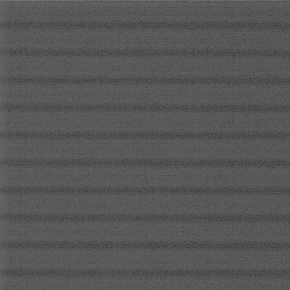
\includegraphics[width=\columnwidth]{20um_vertical_slit_edit_tri.png}
        \caption{縦スリットを置いたとき}
        \label{fig:vslit}
    \end{subfigure}
    \begin{subfigure}{0.4\columnwidth}
        \centering
        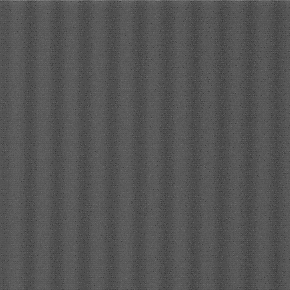
\includegraphics[width=\columnwidth]{20um_horizontal_slit_edit_tri.png}
        \caption{横スリットを置いたとき}
        \label{fig:hslit}
    \end{subfigure}    
    \caption{空間フィルタを置いたときの格子縞の回折像(パターンを見やすくするため画像を補正した.)}
    \label{fig:filter}
\end{figure}

\begin{figure}[htbp]
    \centering
    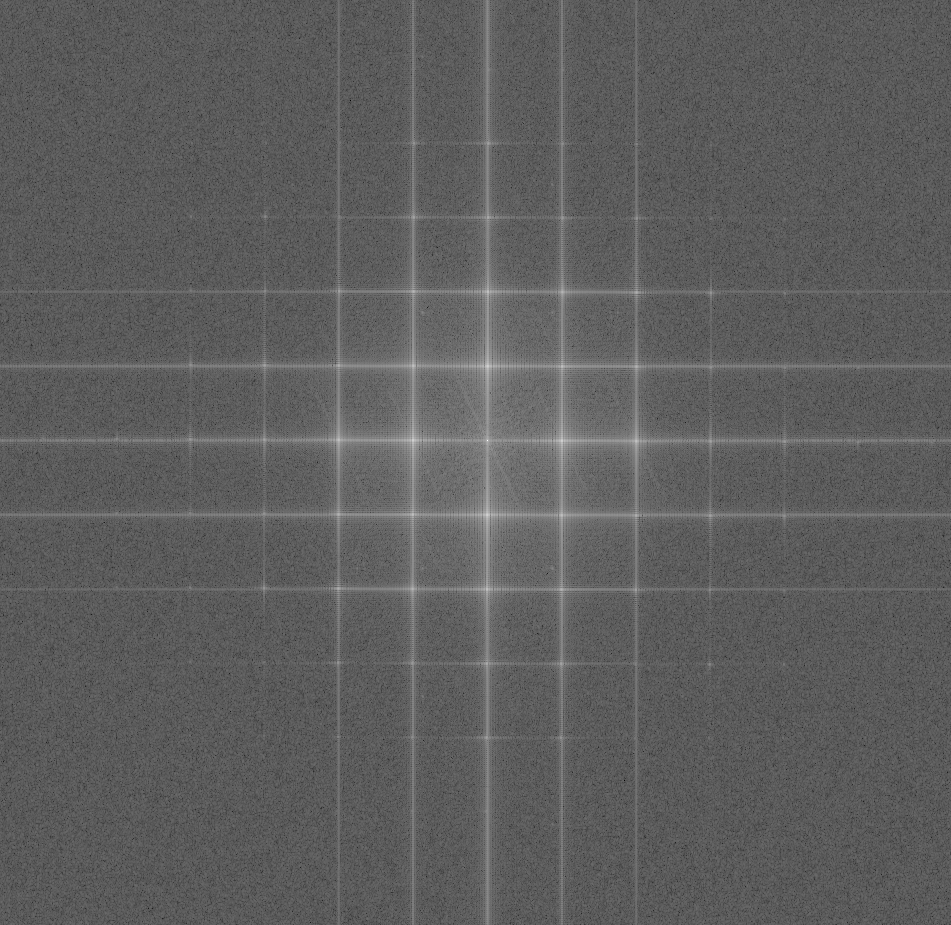
\includegraphics[width=7cm]{FFT_of_20um_blue2_tri.png}
    \caption{20\,$\mu$m間隔の格子縞の画像(図\ref{fig:20blue})をフーリエ変換した結果}
    \label{fig:fourier_direct}
\end{figure}

\begin{figure}[htbp]
    \centering
    \begin{subfigure}{0.38\columnwidth}
        \centering
        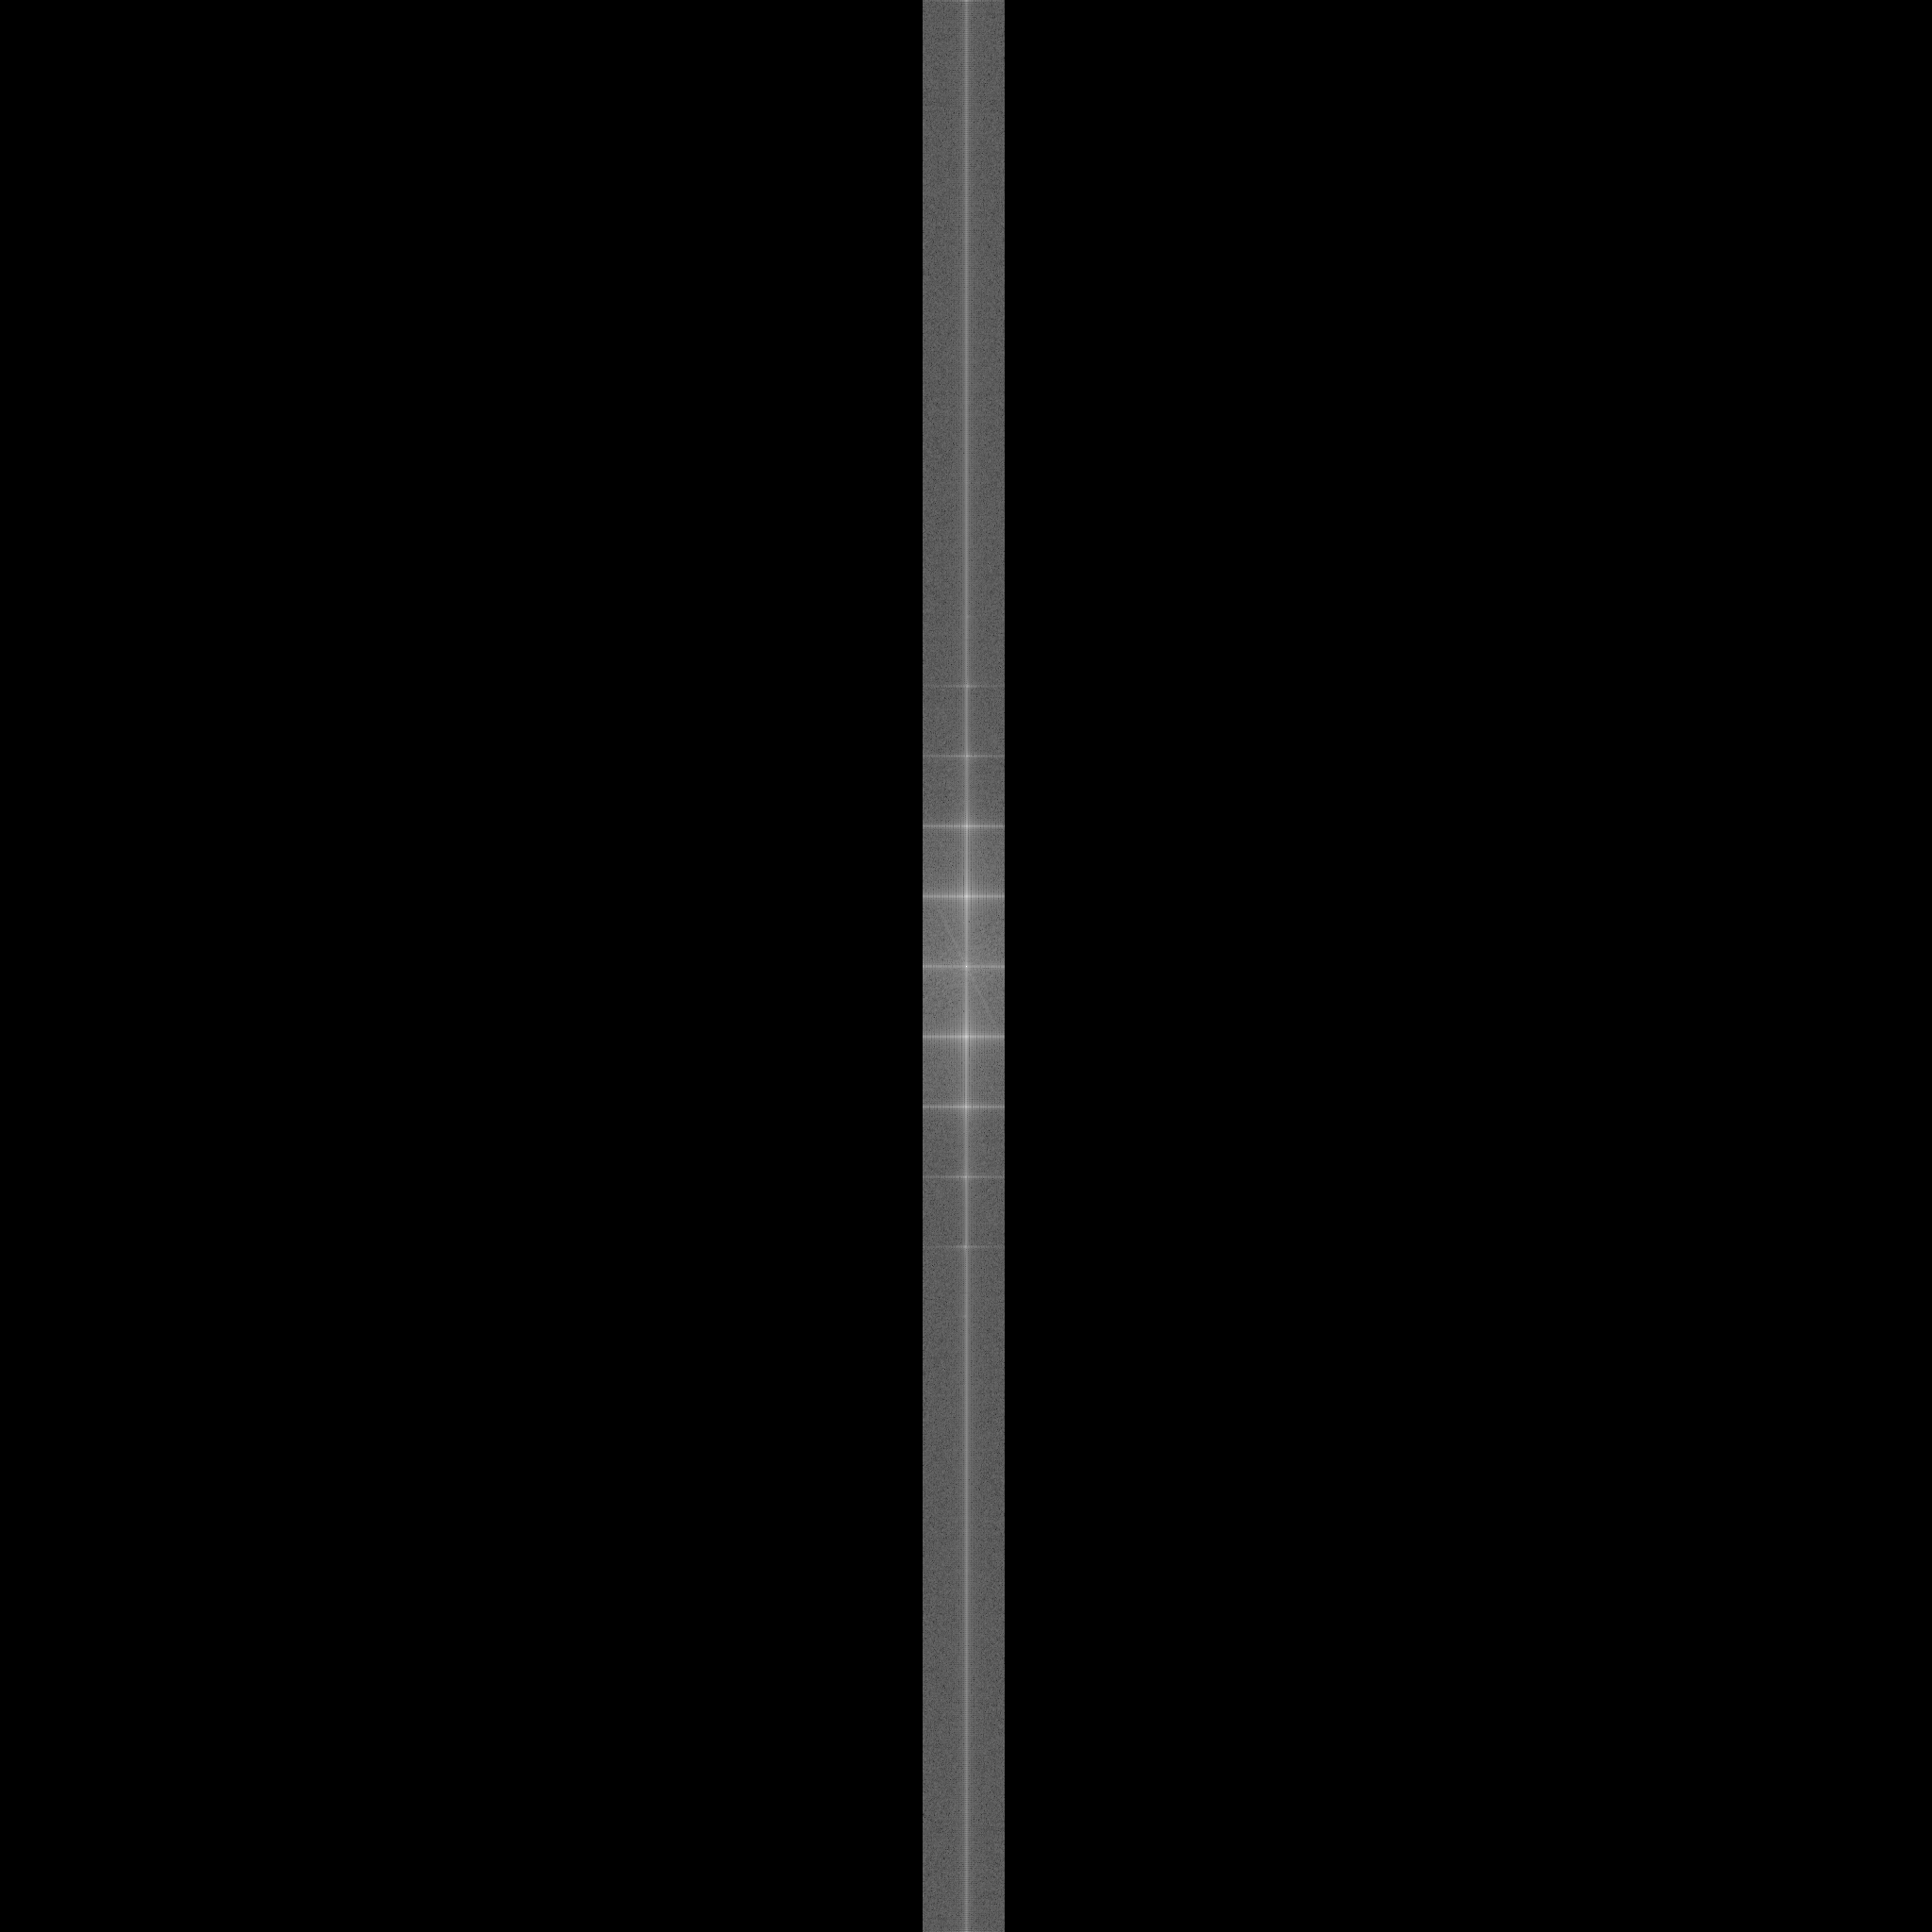
\includegraphics[width=\columnwidth]{20um_blue2_fft_vfilter.png}
        \caption{縦スリットの空間フィルタ}
        \label{fig:fourier_vslit_filter}
    \end{subfigure}
    \begin{subfigure}{0.38\columnwidth}
        \centering
        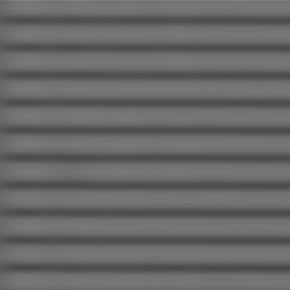
\includegraphics[width=\columnwidth]{20um_blue2_fft_vfilter_invfft_tri.png}
        \caption{左図をフーリエ変換した結果}
        \label{fig:fourier_vslit}
    \end{subfigure}
    \begin{subfigure}{0.38\columnwidth}
        \centering
        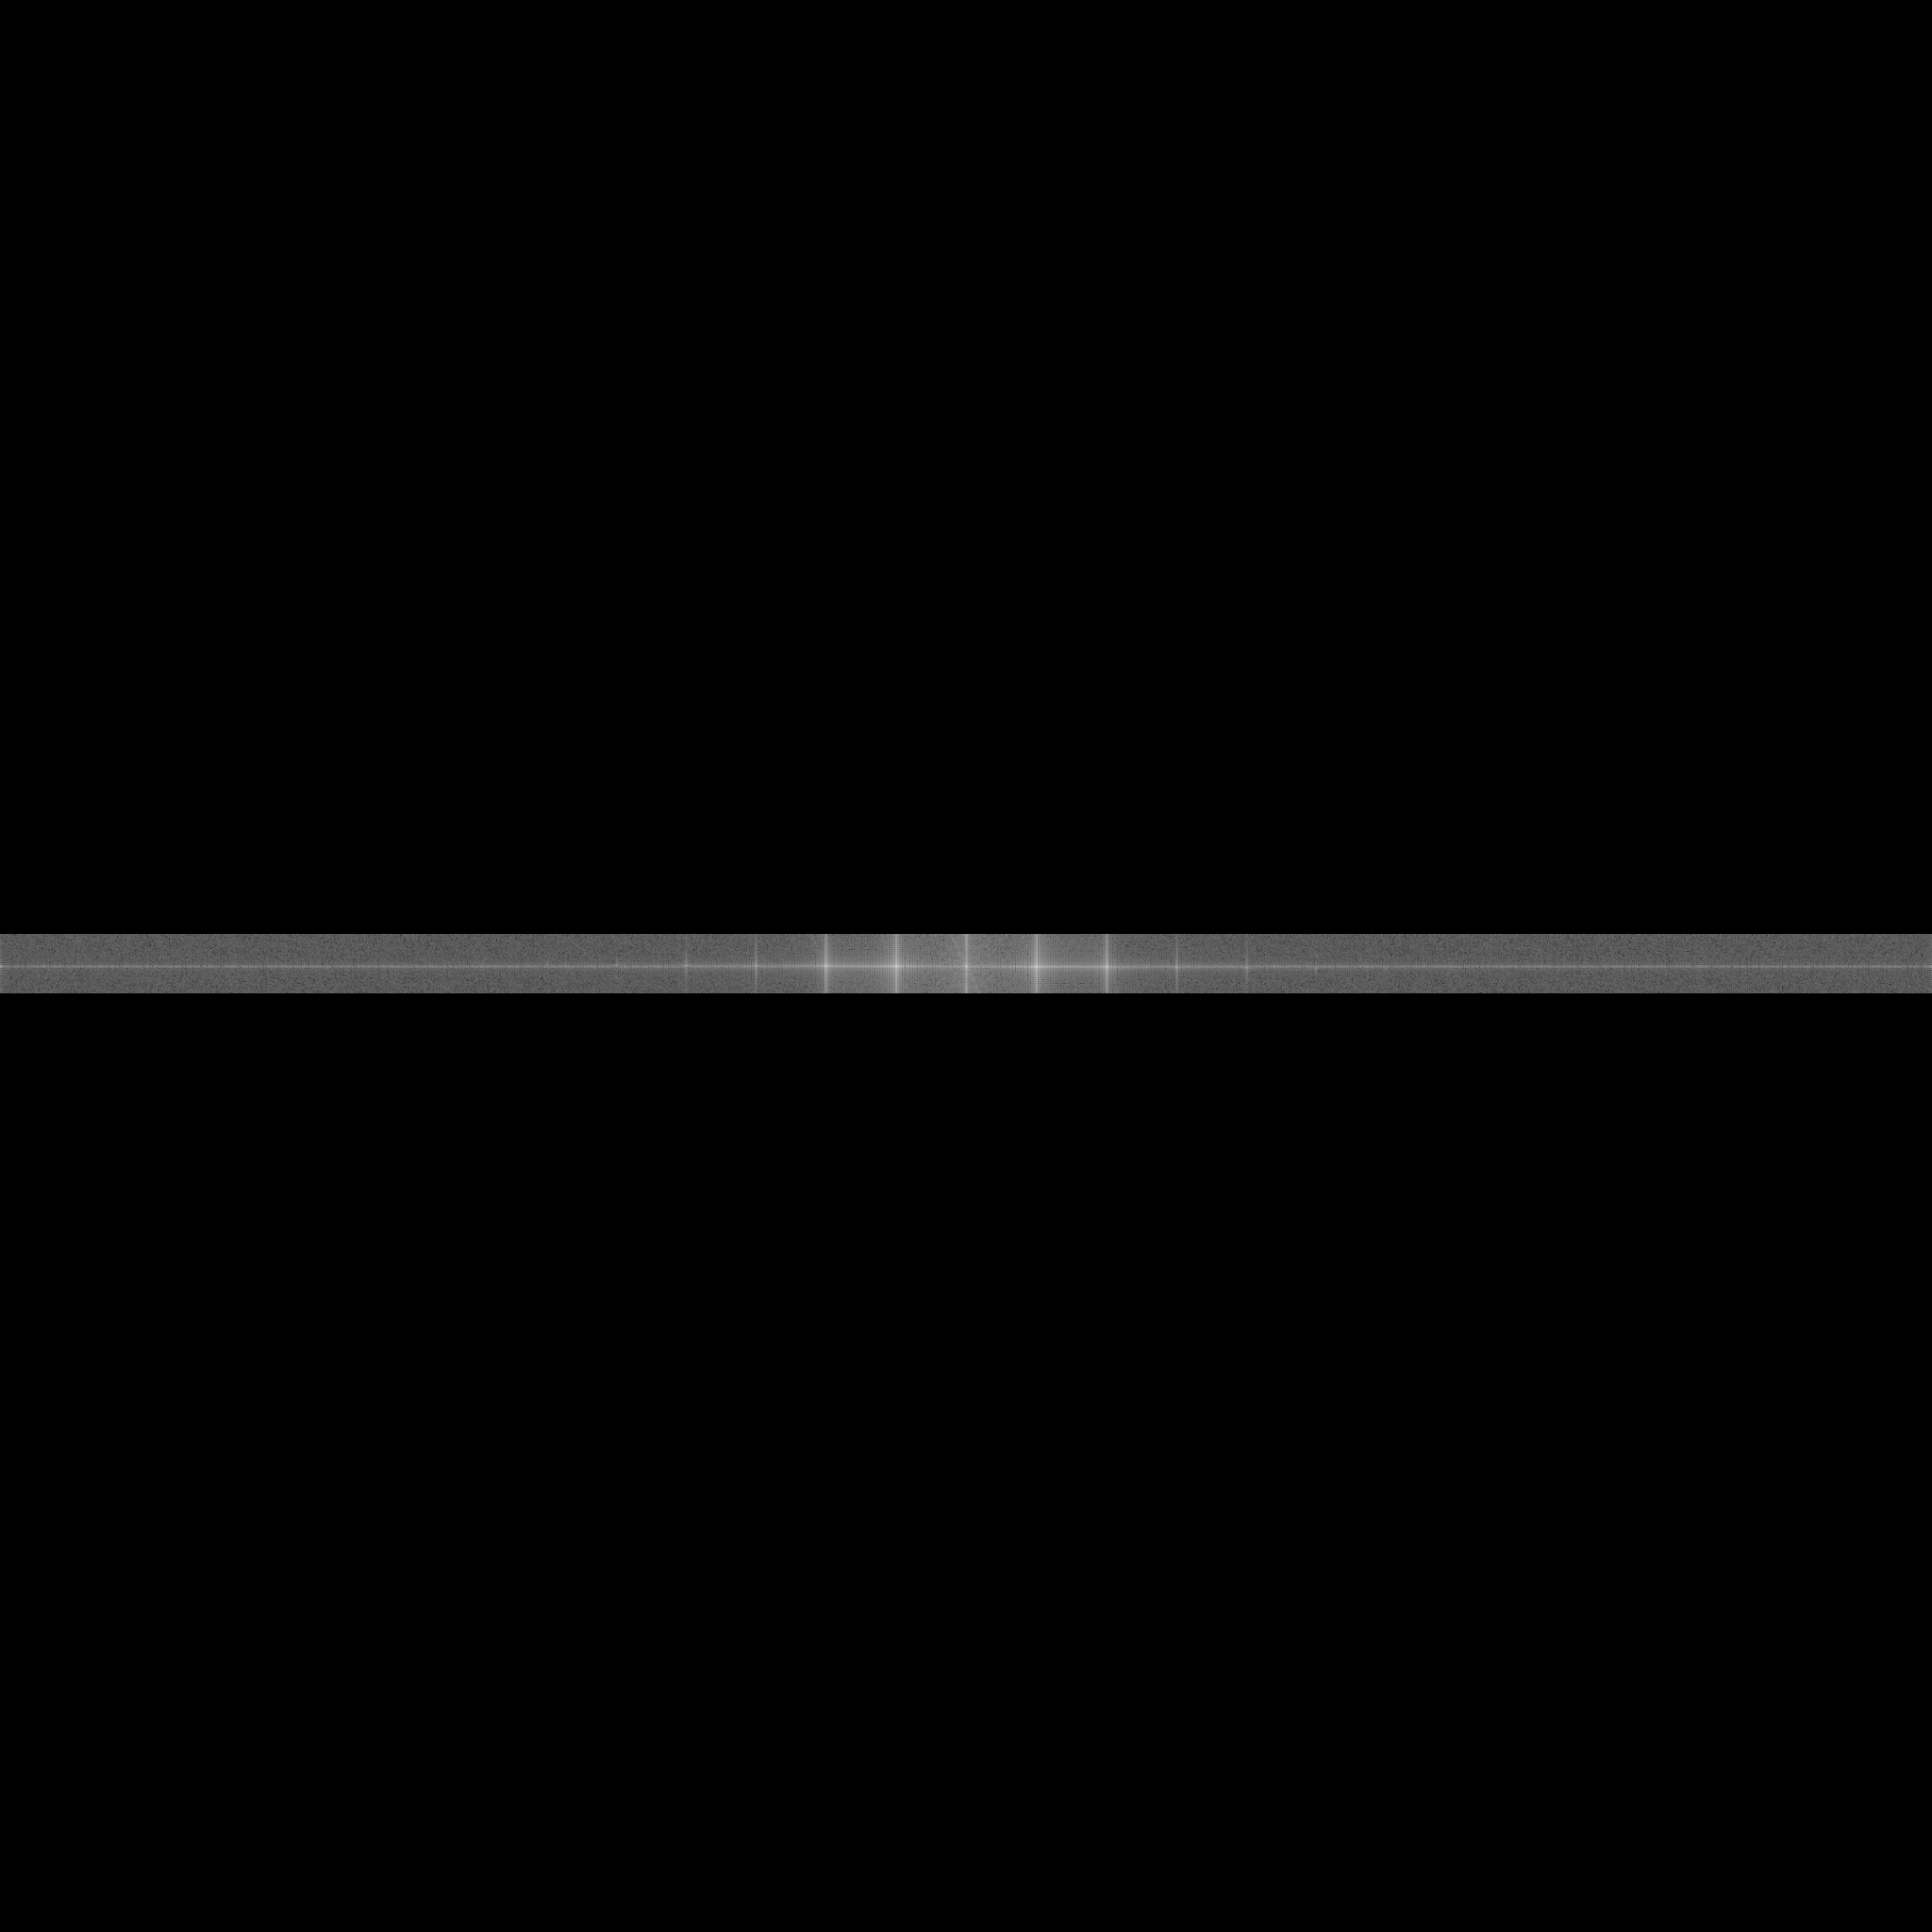
\includegraphics[width=\columnwidth]{20um_blue2_fft_hfilter.png}
        \caption{横スリットの空間フィルタ}
        \label{fig:fourier_hslit_filter}
    \end{subfigure}
    \begin{subfigure}{0.38\columnwidth}
        \centering
        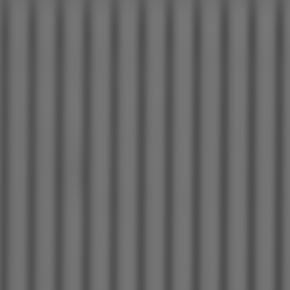
\includegraphics[width=\columnwidth]{20um_blue2_fft_hfilter_fft_tri.png}
        \caption{左図をフーリエ変換した結果}
        \label{fig:fourier_hslit}
    \end{subfigure}
    \begin{subfigure}{0.38\columnwidth}
        \centering
        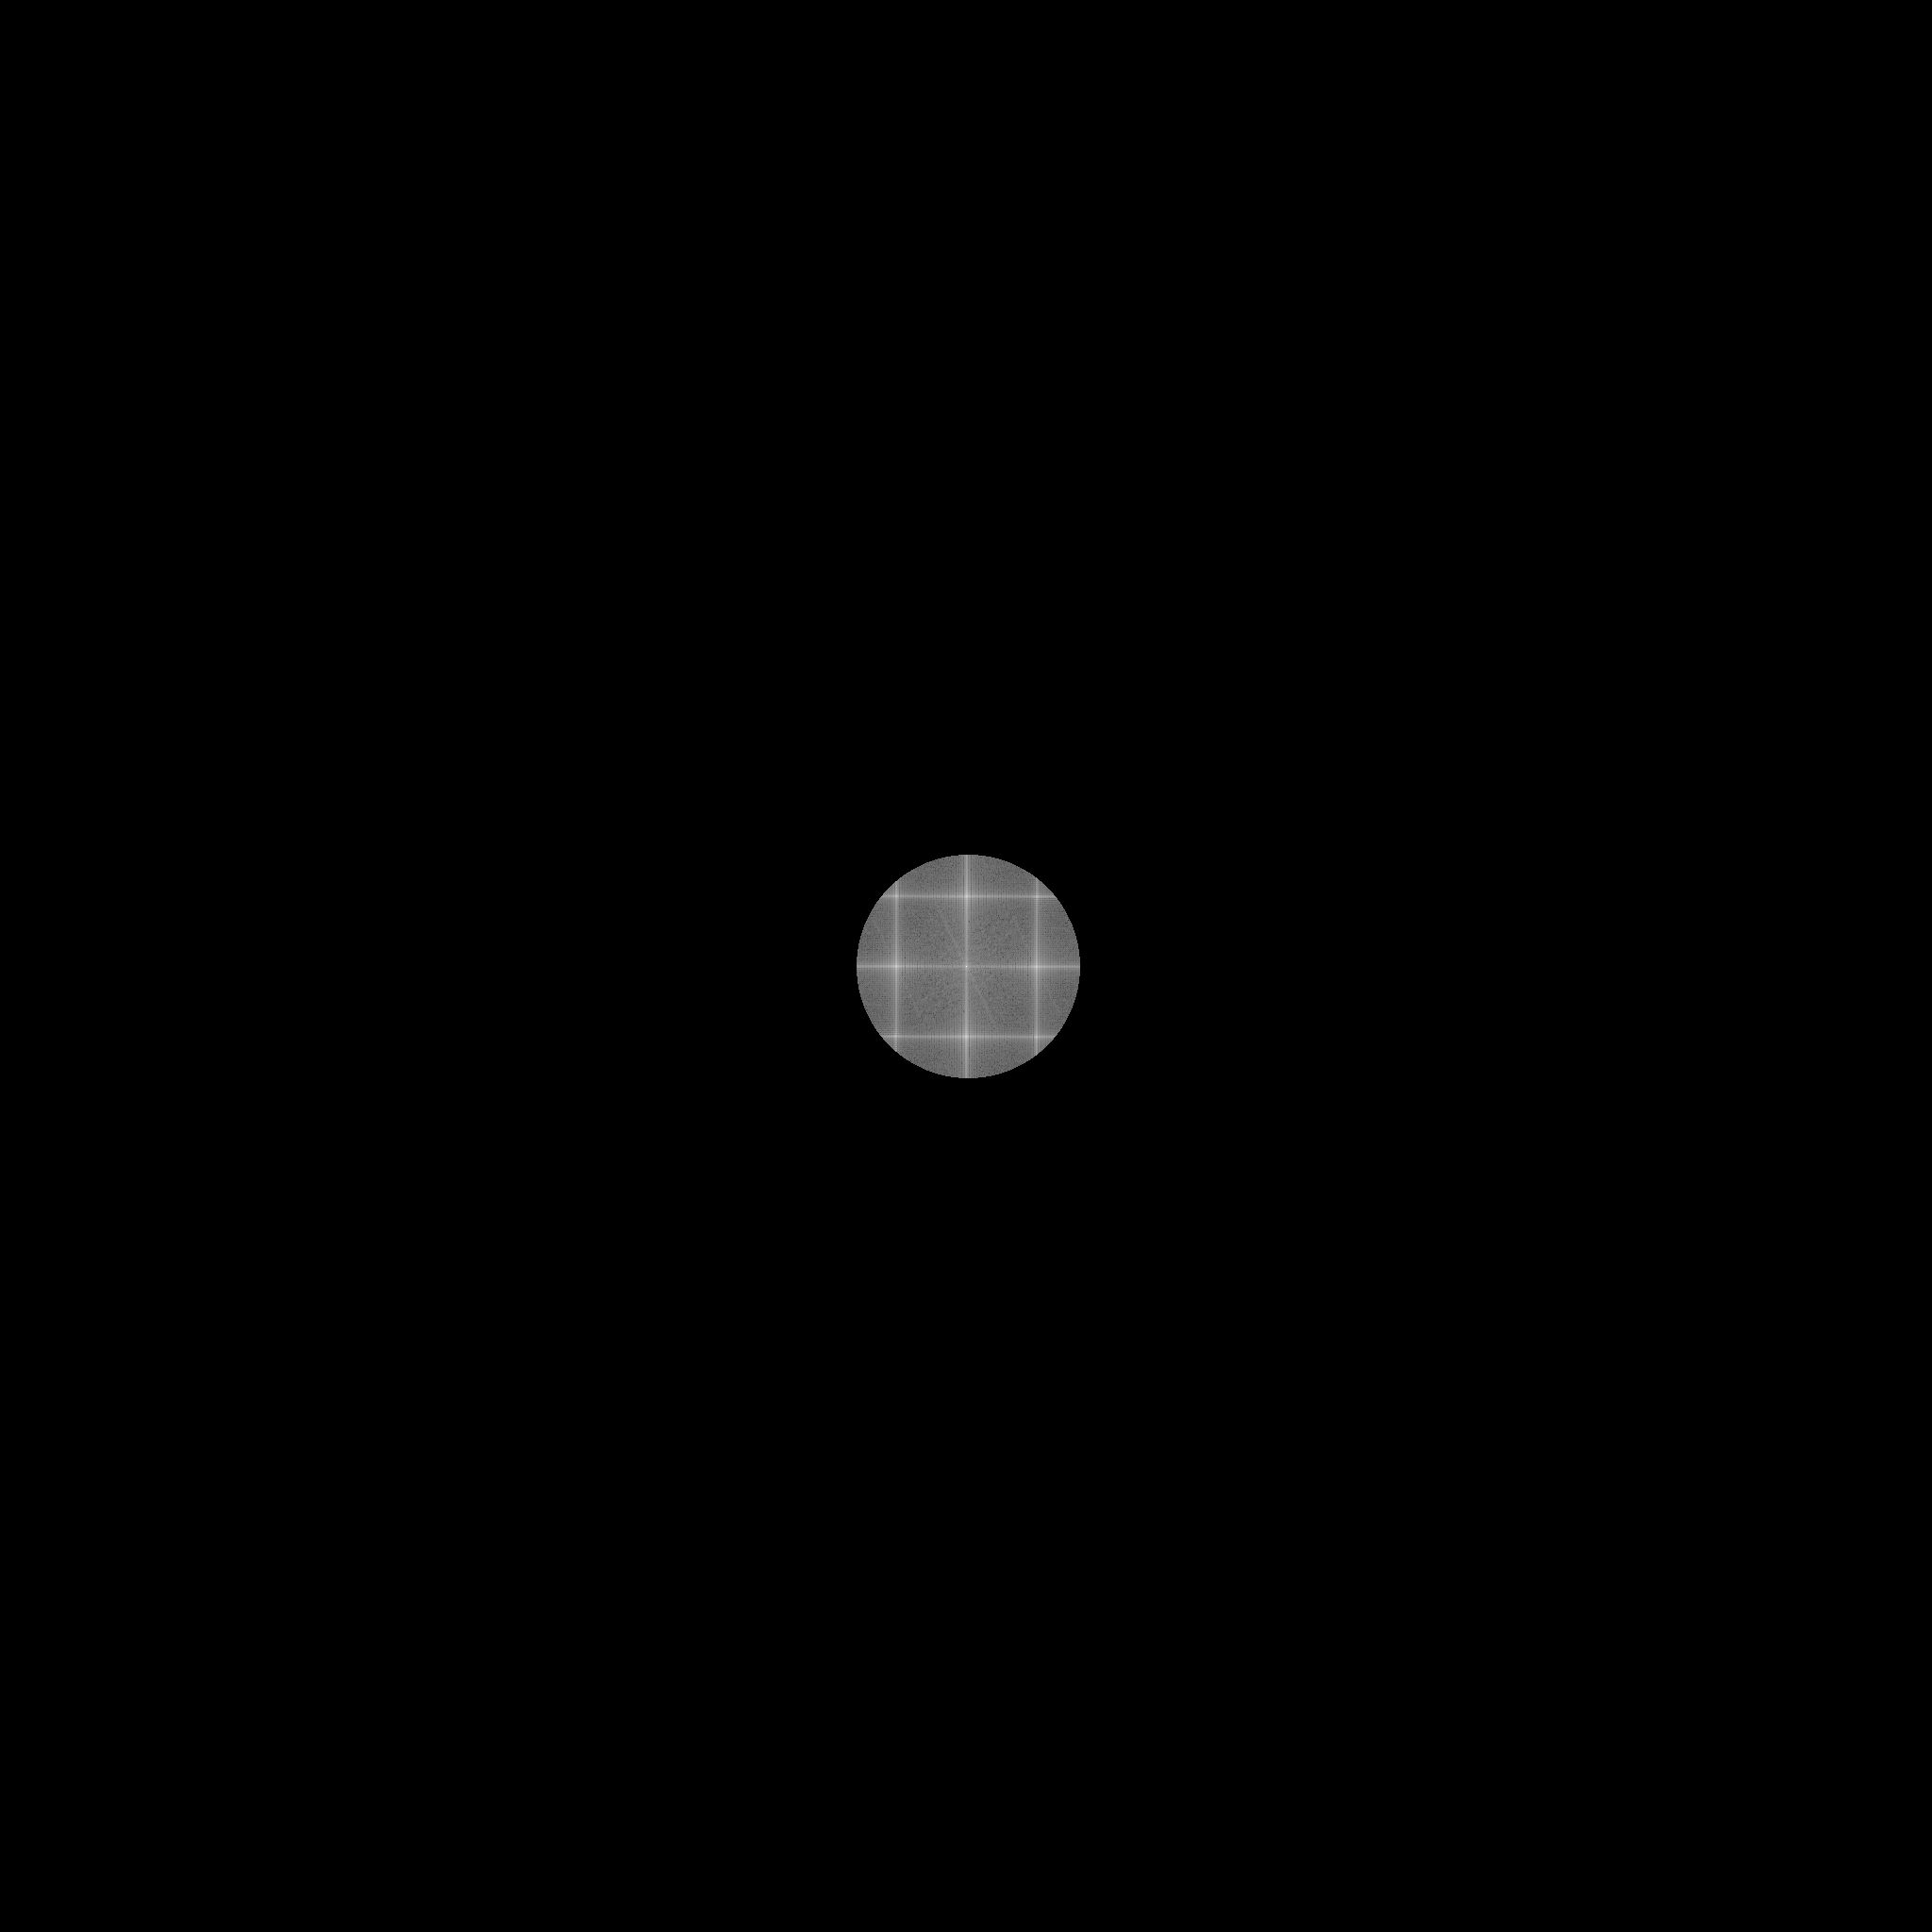
\includegraphics[width=\columnwidth]{20um_blue2_fft_filter3.png}
        \caption{円形フィルタ}
        \label{fig:fourier_circle_filter}
    \end{subfigure}
    \begin{subfigure}{0.38\columnwidth}
        \centering
        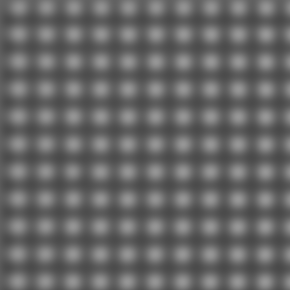
\includegraphics[width=\columnwidth]{20um_blue2_fft_filter3_fft_tri.png}
        \caption{左図をフーリエ変換した結果}
        \label{fig:fourier_circle}
    \end{subfigure}  
    \caption{図\ref{fig:fourier_direct}に空間フィルタを入れて再度フーリエ変換した結果}
    \label{fig:fourier}
\end{figure}

\begin{table}[htbp]
    \centering
    \caption{画像上のスポット間隔の測定値と理論値の比較.光の波長$\lambda =450\,$nm,対物レンズの焦点距離$f=70$\,mm,また画像の1\,pxが実際には5.2\,$\mu$mに対応することを用いた.}
    \label{tab:spot}    
    \begin{tabular}{cc|c}
        格子縞の間隔($\mu$m) & スポットの間隔の理論値($\mu$m) & スポットの間隔の測定値($\mu$m)\\
        \hline\hline
        20 & 1,575 & 1,500\\
        100 & 315 & 310 \\
        \hline
    \end{tabular}
\end{table}

まず20\,$\mu$mおよび100\,$\mu$mの間隔の格子縞の回折像には格子状にスポットが並んでいた(図\ref{fig:spots}).
そのスポットの間隔をImageJ上で測定した(表\ref{tab:spot}).
次に対物絞りの位置に空間フィルタを置いて20\,$\mu$m間隔の格子縞を撮影した結果,縦スリットを置くと横縞が現れ,横スリットを置くと縦縞が現れたことが確認できた(図\ref{fig:filter}).
また実験5で撮影した画像(図\ref{fig:20blue})をフーリエ変換した結果は図\ref{fig:fourier_direct}となった.
またこれに縦スリット・横スリットの空間フィルタを入れて再びフーリエ変換した結果を図\ref{fig:fourier}に示した.
加えて実験5の考察のため円形の空間フィルタを入れてフーリエ変換した結果も同図に示した.

\subsection{考察}
まず最初に撮影した画像\ref{fig:20fourier}は対物レンズによる回折像なので,先述した議論によりこれは理論的には格子縞のフーリエ変換となる.
実際これは図\ref{fig:fourier_direct}の最も明るい部分と対応している.
原点が非常に明るくなっているのは,照明光が瞳面で集光するためと考えられる(図\ref{fig:4fsystem}参照).
この対応関係を原理に立ち戻って考察する.
まず原理で導出した式\eqref{spot}では原点以外のスポットは2箇所しか挙げられていなかったが,今回は格子状に並んだそれ以上の数のスポットが確認できた.
これは格子縞のパターンが一つの余弦波ではなく,複数の余弦波の和の形で書けるためである.
ただしその余弦波はいずれも格子縞の位置に節を持っている必要があるため,その波数は格子縞の間隔に対応する波数の整数倍となっている.
そのため画像上でスポットは格子状に並び,その間隔は$d$を格子縞の間隔としたときに式\eqref{spot}で与えられる長さだと考えられる.
以上と同様のことが図\ref{fig:100fourier}についてもいえる.
また実際に画像上のスポット間の距離を測定し,\eqref{spot}から求めた理論値と比較すると表のように有効数字2桁で一致した.
このことは今の考察が正しいことを裏付ける.

次にカメラを本来の位置に置き,対物絞りの位置に何も置かなかった場合を考える.
原理で述べた通りカメラには格子縞を2回フーリエ変換した像ができる.
ただし2回目のフーリエ変換は空間反転を行うことで$e^{-ikx}$を$e^{ikx}$に変換できるので,1回目のフーリエ変換の逆変換に空間反転を施したものと捉えられる.
そのため格子縞は元通り見えることになる.

続いて対物絞りの位置に空間フィルタを置いた場合を考える.
このとき対物絞りの位置にできた像のうち一部だけが結像レンズによるフーリエ変換を受ける.
そのため1回目のフーリエ変換の一部だけを再びフーリエ変換した像がカメラに映る.
実際,空間フィルタを置いたときの画像(図\ref{fig:vslit},図\ref{fig:hslit})はもとの格子縞の画像(図\ref{fig:20blue})に対してそのようなフーリエ変換を行った画像(図\ref{fig:fourier_vslit},図\ref{fig:fourier_hslit})と同じ模様である.

また空間フィルタとして円の内部のみを透過するものを考え,フーリエ変換を施すと図\ref{fig:fourier_circle}が得られた.
これは実験5で対物絞りを閉じた状況に相当しており,確かに図\ref{fig:fourier_circle}には実験5で得た図\ref{fig:obj_fig}と似たぼやけた格子縞が映っている.
このことはレンズがフーリエ変換を行うという考えから説明できる.
対物絞りの位置にできた格子縞のフーリエ変換は光軸付近から離れるにつれ大きな波数に対応する.
そのため対物絞りを閉じることは格子縞の像の高周波成分をカットすることと等価である.
そして高周波成分が除かれた状態で再びフーリエ変換すると,もとの画像で変動の激しい部分がならされ,輝度分布が滑らかでぼやけた像が得られる.
この像がカメラに映るので,図\ref{fig:obj_fig}は対物絞りを絞る以前よりぼやけていると考えられる.

\section{実験7}
最後に哺乳類細胞の試料を,位相コントラストを振幅コントラストに変換することで見やすく撮影した.

\subsection{原理}
ここでは再び図\ref{fig:4fsystem}を考え,試料として中央部$-w/2<x<w/2$だけ位相が$\theta$遅れるというものを考える.
このとき試料を通った光の複素振幅は
\begin{equation}
    f(x) = \left(1-\Pi \left(\frac{x}{w}\right) \right) + \exp (-i\theta) \Pi \left(\frac{x}{w}\right)
\end{equation}
となる.ここで矩形関数
\begin{equation}
    \Pi \left(x\right) =
    \left\{ 
    \begin{array}{ll}
        1 & -1/2 < x < 1/2\\
        0 & \text{それ以外}
    \end{array}
    \right.
\end{equation}
を用いた.
いま$\theta \ll 1$として
\begin{equation}
    f(x) = 1 - i\theta \Pi \left(\frac{x}{w}\right)
\end{equation}
がいえると考える.
これより瞳面ではこれをフーリエ変換した
\begin{equation}
    F(u) = \delta (u) - iw\theta \,\mathrm{sinc}\left(\frac{uw}{2}\right) 
\end{equation}
というパターンが結像する.
さらに試料からスクリーンに至るまでの経路の途中で位相変化がある場合を考える.
たとえば瞳面に大きさ$\delta$の微小な孔の空いたガラス板を置き,ガラス板を通過した光の位相を$\lambda/4$だけ遅らせるとする.
このとき位相板による位相変化は
\begin{equation}
    H(u) = i + (1-i)\Pi \left(\frac{u}{\delta}\right)
\end{equation}
で与えられる.
このとき瞳面で位相板を通過した後の複素振幅は
\begin{equation}
    HF = \left(i + (1-i)\Pi \left(\frac{u}{\delta}\right)\right)\left(\delta (u) - iw\theta \,\mathrm{sinc}\left(\frac{uw}{2}\right)\right)
\end{equation}
となる.
よってスクリーンでの像はこれをフーリエ変換して実部をとった
\begin{equation}
    1 + \theta \Pi\left(\frac{x}{w}\right) - \frac{2}{\pi}\Pi\left(\mathrm{Si}\left(\frac{\delta}{2}\left(x - \frac{w}{2}\right)\right) - \mathrm{Si}\left(\frac{\delta}{2}\left(x + \frac{w}{2}\right)\right)\right)
    \label{phase}
\end{equation}
と分かる.
ここで正弦積分
\begin{equation}
    \mathrm{Si}(x) = \int_0^x \mathrm{sinc}(t) dt
\end{equation}
を用いた.
式\eqref{phase}を図示すると図\ref{fig:phase}のようになる.
これより試料面の位相差が強度差としてスクリーン上に現れることが分かる.

\begin{figure}[htbp]
    \centering
    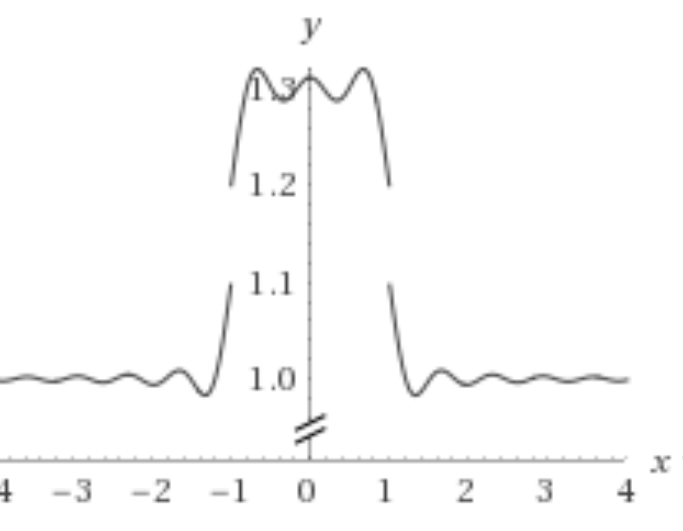
\includegraphics[width=10cm]{phase.png}
    \caption{スクリーンにできる像のパターン}
    \label{fig:phase}
\end{figure}

\subsection{手法}
まず実験5の光学系でコンデンサー絞りを開いて,試料を哺乳類細胞(HeLa cell)に交換し, 像のフォーカスを合わせて撮影した.
このときフォーカスは細胞が背景に溶け込む(コントラストがかからない)ように調整した.
その状態からカメラ位置を前後させたときの画像を撮影した.
またコンデンサー絞りを直径10\,mmに閉じたときにも同様の撮影を行った.

\subsection{結果}
\begin{figure}[htbp]
    \centering
    \begin{subfigure}{0.3\columnwidth}
        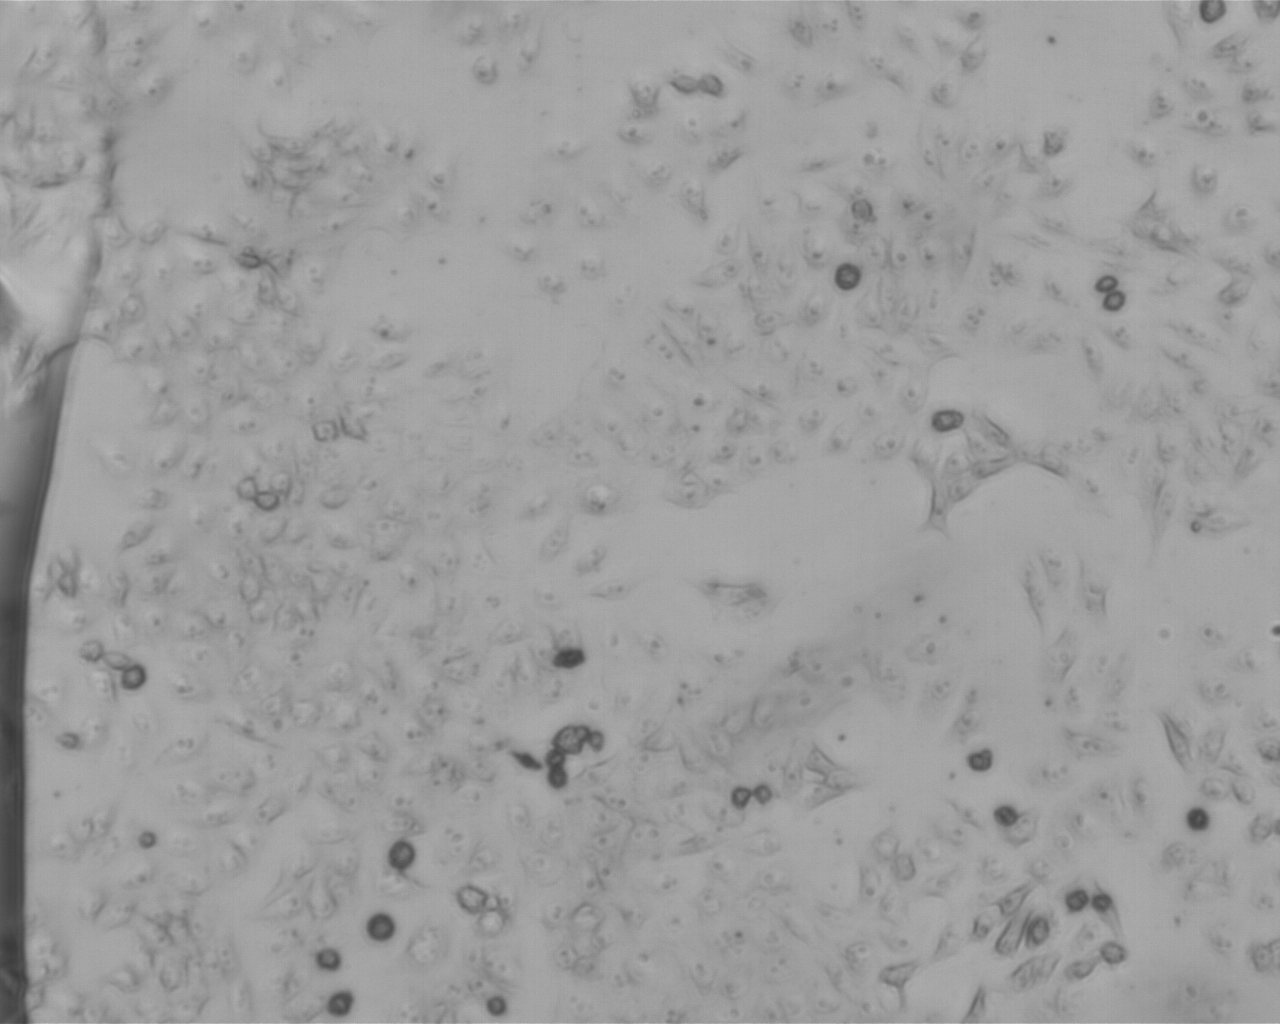
\includegraphics[width=\columnwidth]{1_1_hela.png}
        \caption{フォーカスを合わせた状態}
        \label{fig:1_1_hela}
    \end{subfigure}
    \begin{subfigure}{0.3\columnwidth}
        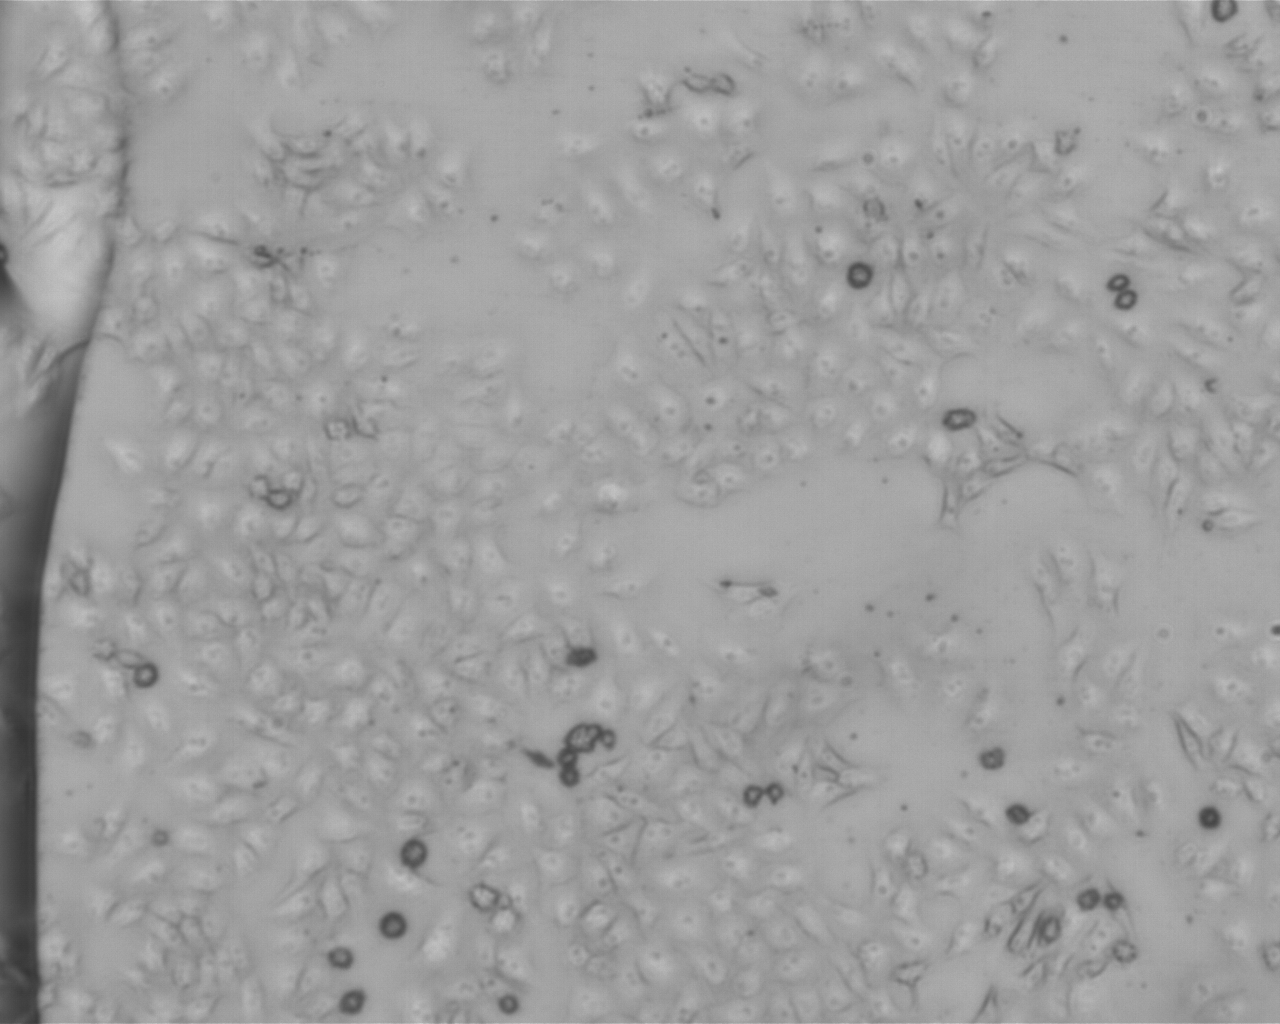
\includegraphics[width=\columnwidth]{1_2_hela_back.png}
        \caption{カメラを後ろに動かした状態}
        \label{fig:1_2_hela}
    \end{subfigure}
    \begin{subfigure}{0.3\columnwidth}
        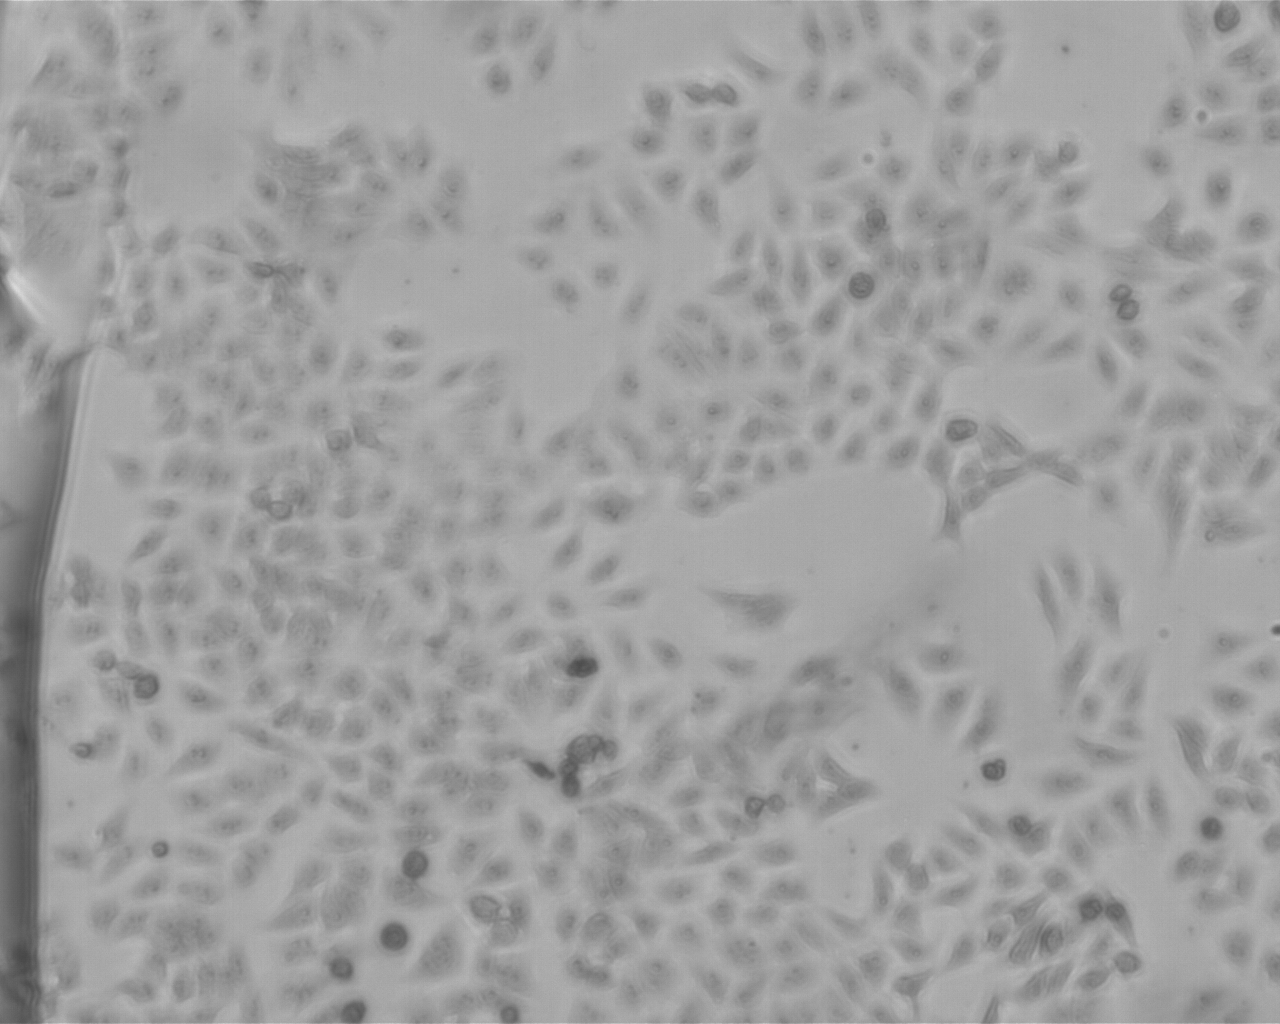
\includegraphics[width=\columnwidth]{1_3_hela_forward.png}
        \caption{カメラを前に動かした状態}
        \label{fig:1_3_hela}
    \end{subfigure}
    \caption{コンデンサー絞りを開いたときのHeLa細胞の画像}
    \label{fig:1_hela}
\end{figure}

\begin{figure}[htbp]
    \centering
    \begin{subfigure}{0.3\columnwidth}
        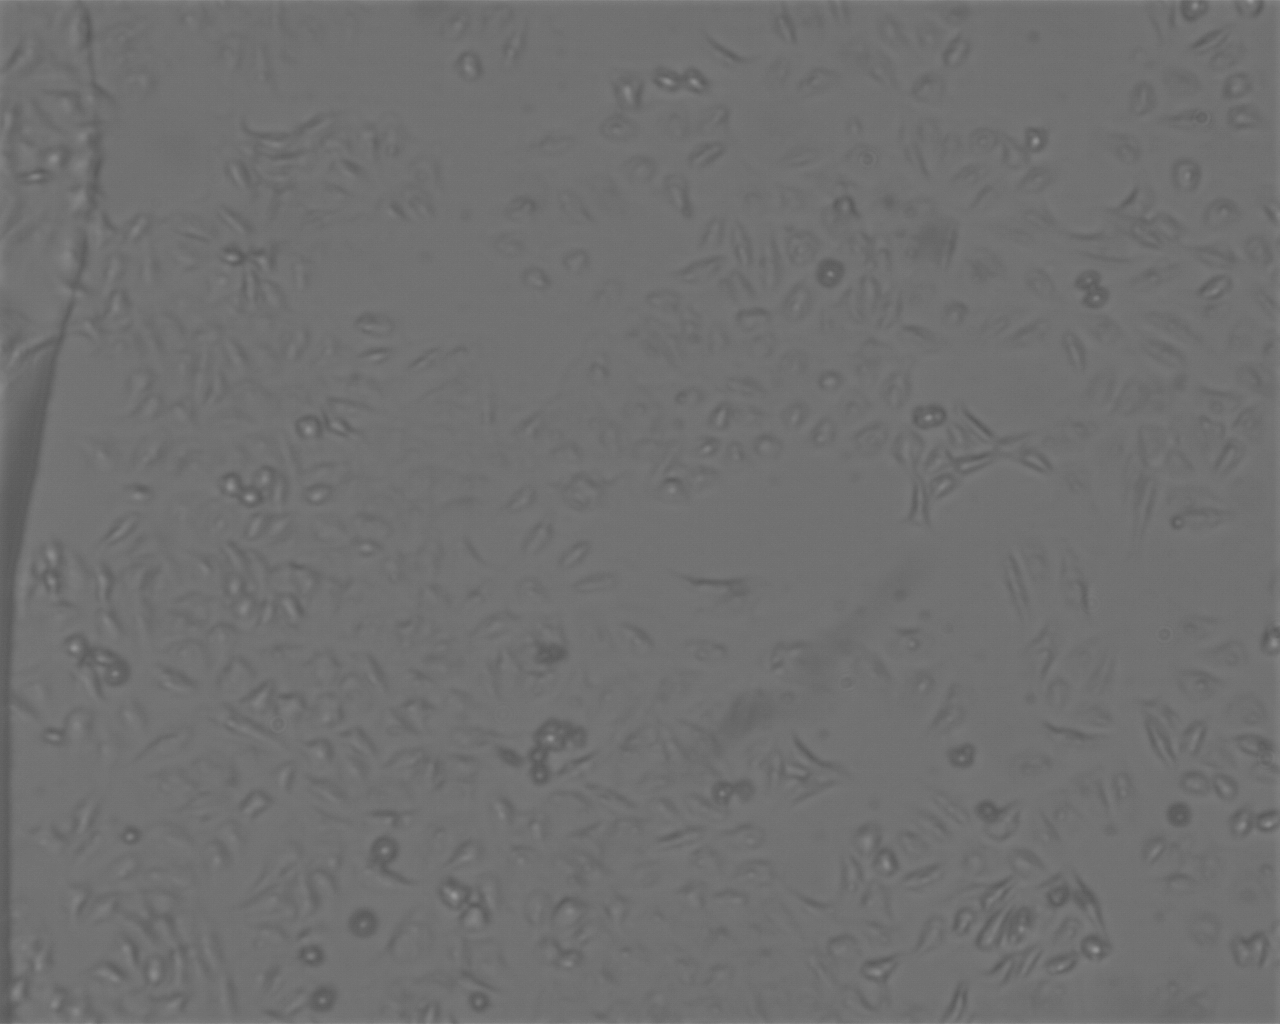
\includegraphics[width=\columnwidth]{2_1_10mm_hela_edit.png}
        \caption{フォーカスを合わせた状態}
        \label{fig:2_1_hela}
    \end{subfigure}
    \begin{subfigure}{0.3\columnwidth}
        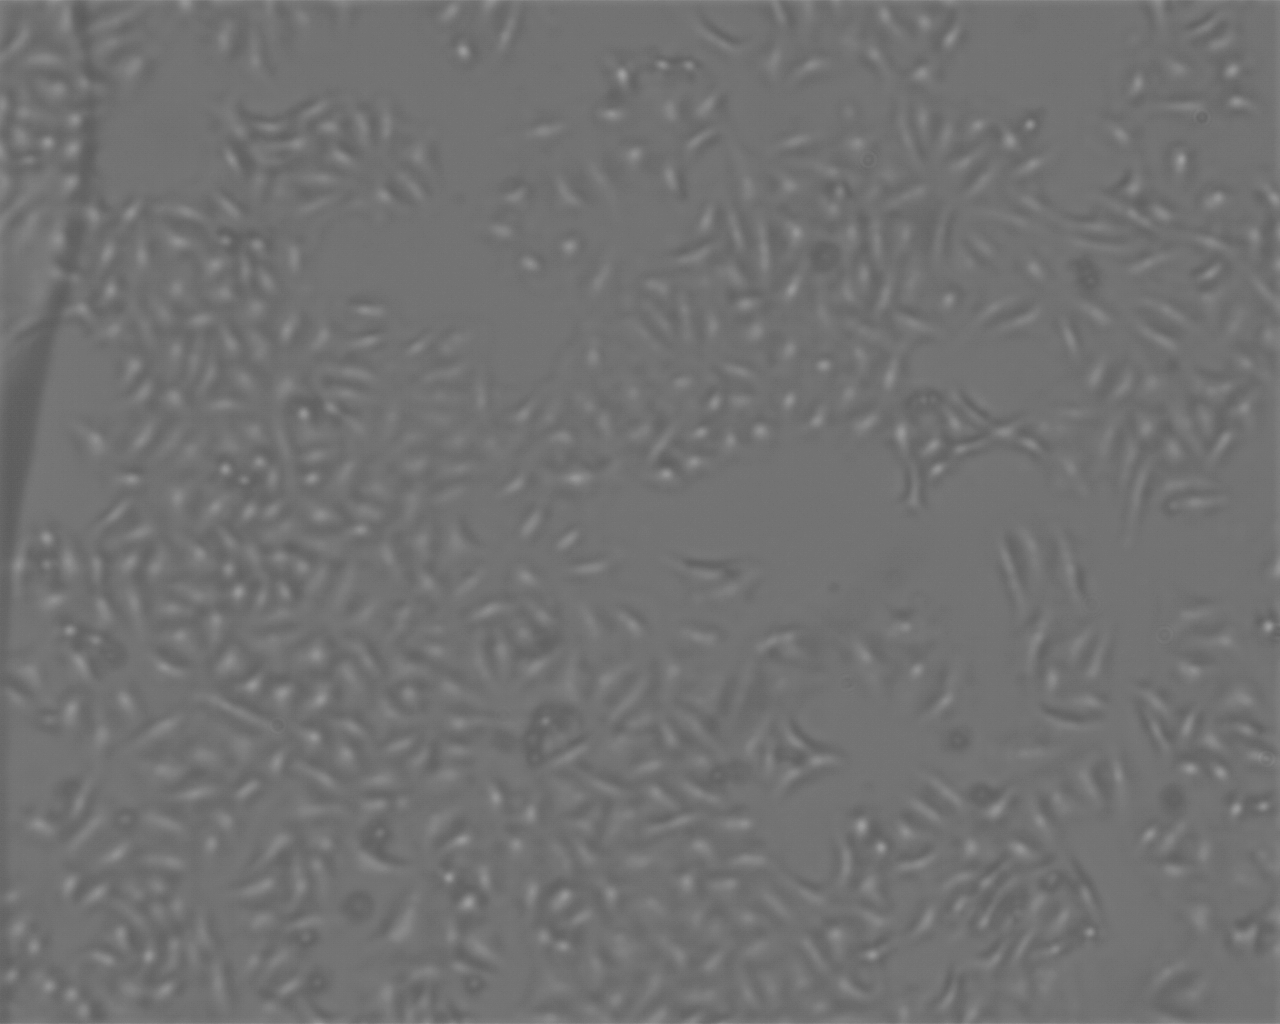
\includegraphics[width=\columnwidth]{2_2_10mm_hela_back_edit.png}
        \caption{カメラを後ろに動かした状態}
        \label{fig:2_2_hela}
    \end{subfigure}
    \begin{subfigure}{0.3\columnwidth}
        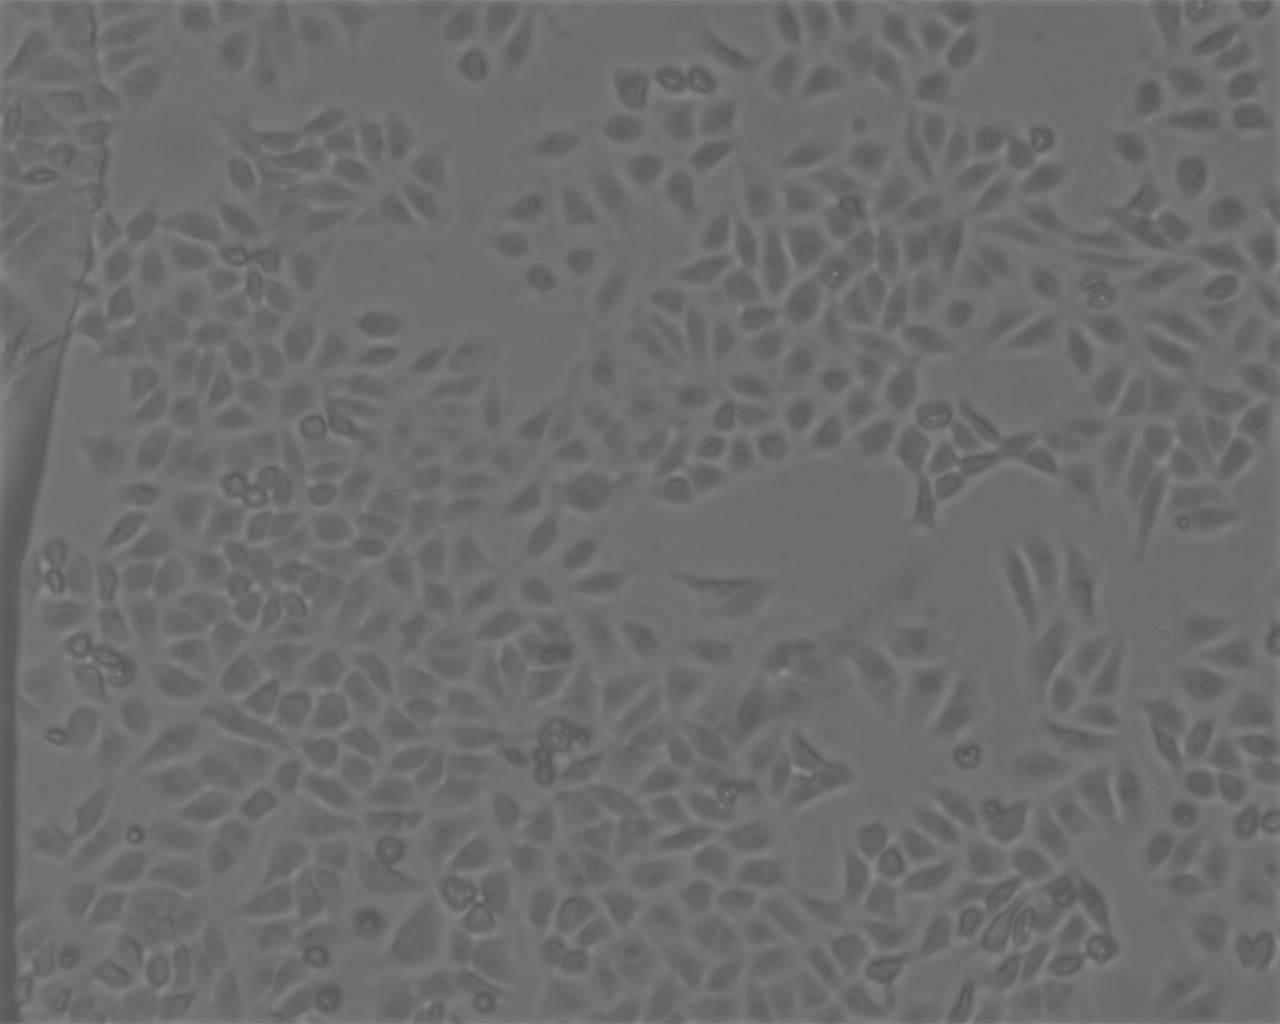
\includegraphics[width=\columnwidth]{2_3_10mm_hela_forward_edit.png}
        \caption{カメラを前に動かした状態}
        \label{fig:2_3_hela}
    \end{subfigure}
    \caption{コンデンサー絞りを10\,mmに閉じたときのHeLa細胞の画像(見やすくするため画像すべてに同じ明るさ補正を施した.)}
    \label{fig:2_hela}
\end{figure}

まずコンデンサー絞りを開いた状態でフォーカスを合わせて撮影したところ,図\ref{fig:1_1_hela}のように細胞が背景とほぼ同色となった.
その後カメラを前後にずらして撮影したところ,図\ref{fig:1_2_hela},図\ref{fig:1_3_hela}のように細胞が縁取られてはっきりと見えるようになった.
ただしこのとき像はぼやけた.
次にコンデンサー絞りを10\,mmに閉じたときにも同様の結果が得られた(図\ref{fig:2_hela}).
またコンデンサー絞りを開いたときと閉じたときで比較すると,コンデンサー絞りを閉じることでどれもコントラストが強まったことが確認できた.
さらにコンデンサー絞りの開閉にかかわらず,カメラを後ろに動かすと細胞は白く見え,カメラを前に動かすと細胞は黒く見えた.

\subsection{考察}

まずカメラを前後させることでコントラストが強まる理由を考察する.
最初にこの実験の原理を参考にしたフーリエ結像に基づく考察を述べ,次に素朴な光線の軌跡に基づく考察を述べる.
前者の考察にはやや問題が残っているが,念のためレポートに載せることにした.
そして最後に光線の軌跡に基づく考察の定量的な裏付けを述べる.

\subsubsection{フーリエ結像に基づく考察}
HeLa細胞は無色透明だが細胞の内外で屈折率が異なるので,細胞を通った光は通らなかった光と比べて位相が変わる.
ところが原理で述べたように,実験5と同じ位置にカメラを置いて撮影してもこの位相差は画像の強度差には現れないので,細胞が無色透明である像が得られる.
原理では瞳面で位相変化を与えることでこの位相差を強度差に変換して投影できることを示した.
今回の実験では同様の位相変化を瞳面ではなくカメラの直前で行っており,このときにも同じく位相コントラスト像が見られることを示す.

カメラを後方に距離$d$だけわずかに移動させると,光軸から距離$r$にあるカメラ上の点に到達する光の位相は光軸に沿って到達する光に比べて位相が
\begin{equation}
    k(\sqrt{d^2 + r^2} - d) \approx \frac{k r^2}{2d}
    \label{cameraphase}
\end{equation}
だけ遅れる.
このときカメラに映る像は瞳面のフーリエ変換にこの位相変化に対応する位相因子を掛けたものになると考えられる\footnote{カメラを移動させるとカメラ上で光は結像しないのでフーリエ結像の議論は厳密には成り立たないが,ここではカメラの移動距離が短いと考え,カメラ上でフーリエ結像が起こるとした.}.
このフーリエ変換の積分変数は瞳面の座標であり位相因子とは無関係なので,位相因子を瞳面の強度分布にあらかじめ掛けておきそれをフーリエ変換しても同じ結果が得られる.
後者の計算では位相変化は原理で述べた$H(u)$と同じように捉えることができるため,同様の議論により試料の位相差が画像の強度差に変換される.
前方に移動させる場合も$d<0$とすれば同様に考えることができる.

またカメラを後ろに動かすと光軸から離れた位置に達する光の位相が遅れるが,前に動かすとそれは逆に進むことになる.
このことからカメラを前に動かすことは,原理で述べた例でいえば位相板が光の位相を$\lambda /4$だけ早める場合に対応する.
この場合に原理で行った計算をやり直すと,スクリーンにできるパターンは中央がへこんだ形となる.
つまり試料上の位相を遅らせる部分は周囲より暗く映ることになる.
今回の実験でカメラを前に動かした際に細胞が暗く映ったのは,これと同様の理由と考えられる.

\subsubsection{光線の軌跡に基づく考察}
上の考察は本来結像していない地点でフーリエ結像の議論を用いているという問題がある上,結局のところ何が起きているのか分かりづらい.
そこで図\ref{fig:obj_fig}に立ち戻ってサンプルからカメラに届く光線に注目して考える.

まず図\ref{fig:obj_fig}から,カメラに到達する光線はカメラ面にほぼ垂直に入射するものと斜めに入射するものに分けられることが分かる.
ただしカメラの同じ位置に到達する光線はサンプル上の同じ位置に由来している.
ところがカメラを後ろに動かすと,ほぼ垂直に入射するものはもともととほぼ同じ位置に入射する一方,斜めに入射するものはもととずれた位置に入射する.
そのためこのときカメラの各点では,先ほどと同じサンプル位置から届いた光(直接光)と,異なるサンプル位置から届いた光(回折光)が混じることになる.
カメラ上ではこの直接光と回折光が干渉し,光が強め合う部分は明るく映り,光が弱め合う部分では暗く映る.
強め合うか弱め合うかは直接光と回折光の位相差によって決まるが,その位相差にはカメラを動かすことによる分のほかにサンプル上で細胞を通過することによりついた分がある.

具体的にカメラ上の位置Aを考え,そこにはある細胞を通過した光が直接光として届き,その細胞のすぐ外側から来た光が回折光として届くとする.
このときカメラを後ろに動かすことで回折光の位相が遅れ,その遅れが細胞を通過したことによる直接光の遅れと一致した場合,カメラ上でこれらの光は同位相となり強め合う.
一方カメラ上でそのすぐ隣には,その細胞のすぐ外側の光が直接光となり,その細胞を通過した光が回折光となる位置Bがある.
そこでは細胞を通過したことで遅れた回折光の位相がカメラを後ろに動かすことでさらに遅れる.
そのため直接光と位相がずれ,光は干渉して弱め合う.
その結果,カメラ上で細胞の像はより明るく,その周囲はより暗く見え,コントラストがつく.

逆にカメラを前に動かすと,位置Aでは回折光の位相が進み,それによって直接光と回折光の位相がずれてくると光は干渉して弱め合う.
一方位置Bでは細胞を通過したことで遅れていた回折光の位相が進んで相殺し,直接光とほぼ同じ位相になって光は強め合う.
その結果,カメラ上で細胞の像がより暗く,その周囲は明るく見え,先ほどと逆のコントラストがつく.

この考察はコントラストの付き方も含めて今回の実験結果と合致する.

\subsubsection{光線に基づく考察の定量的裏付け}
光線に基づく考察では細胞を通過することによる位相のずれとカメラを動かすことによる位相のずれを同程度とした.
最後にそれが妥当であることを示す.

図\ref{fig:1_2_hela}の画像から細胞は約50\,pxを占めている.
よって長さに換算するとカメラ上で細胞の像の大きさは$r\approx 250\,\mu$mとなる.
今回顕微鏡の結像光学系は試料を$500/70$倍に拡大しているので,もとの細胞の大きさは$250\times 70/500 \,\mu\mathrm{m}= 35\,\mu\mathrm{m}$と分かる.
よって細胞(屈折率は水と同じくらいの$n\approx 1.34$\footnote{参考文献\cite{nenpyo}参照.}とし,厚さはいま見積もった大きさ$L\approx 35\,\mu$mとする)を通過したとき,通過しないときと比べて
\begin{equation}
    l_0 = (n-1)L = 0.35\times 35\,\mu\mathrm{m} \approx 12\,\mu\mathrm{m}
\end{equation}
だけ余分に光路長が伸びる.

\begin{figure}[htbp]
    \centering
    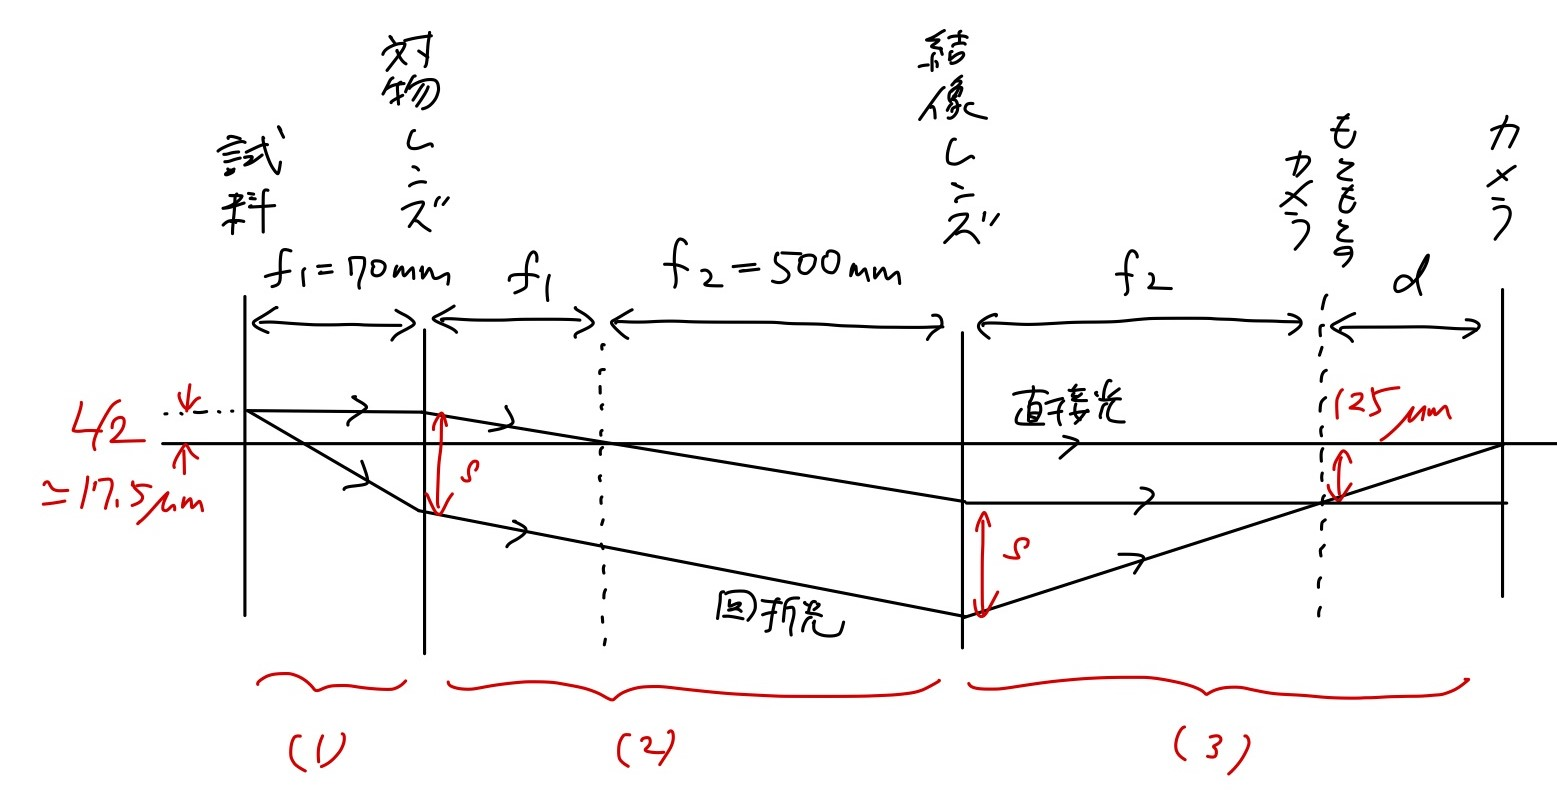
\includegraphics[width=14cm]{objphase.jpg}
    \caption{カメラを距離$d$だけ後方にずらしたときの作図.細胞1個の大きさの半分だけずれた点からの光を回折光としている.距離$s$および三つの区間(1),(2),(3)を図のように定義する.}
    \label{fig:objphase}
\end{figure}

次にカメラを距離$d$だけ動かすことでこれと同じだけ位相をずらすことを考える.
ここで回折光としてサンプル上の細胞1個の大きさの半分(細胞の中央から縁までの大体の距離)だけずれた点から出た光を考える(図\ref{fig:objphase}).
図に示した距離$s$は
\begin{equation}
    s = \frac{f_2}{d}\times 125\,\mu\mathrm{m}
\end{equation}
と求まる.
まず試料から対物レンズまでの区間(1)で,回折光が直接光と比べて余分に進んだ光路長は
\begin{equation}
    l_1 = \sqrt{f_1^2 + s^2} - f_1 \approx \frac{s^2}{2f_1} \approx \frac{28\,\mathrm{mm}^3}{d^2}
\end{equation}
と求まる.
次に対物レンズから結像レンズまでの区間(2)では,
\begin{equation}
    l_2 = \sqrt{(f_1+f_2)^2 + (17.5\,\mu\mathrm{m}+125\,\mu\mathrm{m})^2} - (f_1 + f_2) \approx 18\,\mathrm{nm}
\end{equation}
と求まる.
最後に結像レンズからカメラまでの区間(3)では,
\begin{equation}
    l_3 = \sqrt{(f_2+d)^2 + (125\,\mu\mathrm{m})^2} \approx \frac{s^2}{2f_2} \approx \frac{4\,\mathrm{mm}^3}{d^2}
\end{equation}
と求まる.
よって主要な部分は区間(1),(3)であり,
\begin{equation}
    l_0 = l_1 + l_2 + l_3 \approx \frac{32\mathrm{mm}^3}{d^2} = 12\,\mu\mathrm{m}
\end{equation}
を解くと
\begin{equation}
    d \approx 50\,\mathrm{mm}
\end{equation}
となって確かに今回動かしたカメラの距離とオーダーがおおよそ一致する.
つまり今回のカメラの操作による位相のずれは細胞を通過したことによる位相のずれと同程度であることが分かる.

\section{実験の感想}
実験前に実験の原理をスライドで解説していただけたのはとても助かりました.
実験の種目も多すぎずちょうど良かったと思います.
実験の際のサポートも手厚かったのでありがたかったです.

レポートを書いてみると,数式等を使って定量的に考察する機会が少ない印象でした.(やろうと思えばできたのかもしれません.)
むしろ画像を見て何が起こっているか判断することがメインでしたが,見づらい画像を編集したり,画像の様子をうまく言葉で表現するのが難しかったです.
たとえば「コントラスト」や「解像度」といった言葉を使うのが難しかったので,「はっきりしている」や「ぼやけている」程度のことしか表現できませんでした.
そのため画像から(ImageJなどを用いて)数値の形で情報を引き出す方法などのヒントを冊子に書いていただけると,もう少し明瞭な考察が書けるかもしれないと感じました.

\begin{thebibliography}{99}
\bibitem{text}
   「物理学実験\ajRoman{2}」解説書「顕微鏡光学系」2021年度
\bibitem{nenpyo}
    国立天文台編「理科年表2019」丸善出版
\end{thebibliography}

\end{document}
